Article: Quantile Index for Gradual and Abrupt Change Detection from CFB Boiler Sensor Data in Online Settings.

\begin{abstract}
In this paper we consider the problem of online detection of gradual and abrupt changes in sensor data having high levels of noise and outliers.
We propose a simple heuristic method based on the Quantile Index (QI) and study how robust this method is for detecting both gradual and abrupt changes with such data.
We evaluate the performance of our method on the artificially generated and real datasets that represent different operational settings of a pilot circulating fluidized bed (CFB) reactor and CFB cold model. 
Our experiments suggest that QI can be used for designing very simple yet effective methods for gradual change detection in the noisy sensor data. It can be also used for detecting abrupt changes in the data unless they occur too often one after another.
\end{abstract}

\section{INTRODUCTION}
Sensor data and their analysis are used to monitor and control various types of processes in the systems.
Detecting changes in the time series signal gathered from the sensor is vital for many applications.
It is important to monitor an industrial process online in order to prevent undesirable process conditions.
For instance in the circulating fluidized bed (CFB) boilers particle size distribution is constantly changing.
Defluidization and insufficient heat transfer may cause an agglomeration of the bed particles.
This kind of events may lead to the shut down of the plant.

It is difficult to design a universal change detection method that would handle well different kinds of data and different kind of changes.
In practice, when designing a change detection algorithm, we need to use \emph{prior information} about the data and the anticipated changes if such information is available~\cite{I.V.Nikiforov}.

The term change point stands for a phenomenon when statistical properties of a data stream change over time.
Many approaches for statistical change (point) detection have been proposed in the literature, e.g.~\cite{Aggarwal05,Dasu06}. Some of them focused or suit particularly well on change detection in time series data, e.g.~\cite{journals/tkde/TakeuchiY06,cusum,BifetG07}.
Most of the proposed approaches rely on statistical change detection based on the monitoring of the changes in the data itself or in the outputs of the models learnt on that data. Most of the approaches are not parameter free and rely on certain assumptions about data, the expected change, and what is known about the possible values of the parameters before and after change~\cite{I.V.Nikiforov}.

In monitoring the operation cycles of the CFB boilers, we may deal with processes where we do not have any prior information, i.e.\ the online detection of change points in the sensor data is often complicated by the fact that data is noisy and may have an unknown dynamics.
In such cases thresholding heuristics often appear to be rather effective for an (abrupt) change detection with noisy data~\cite{ZliobaiteBP09}. 

In this paper, we propose Quantile Index (QI) -- a simple heuristic method based on quantile statistic aiming to handle at the first place the gradual changes in the noisy sensor data.
We focus on two basic cases: change (increase) in the mean and change (increase) in the variance of a noisy signal.

The rest of the paper is organized as follows.
In Section~\ref{sec:problem} we discuss the problem of online change detection in two different tasks -- pressure fluctuation and fuel mass flow estimation from the noisy sensor data.
In Section~\ref{sec:ourapproach} we first consider density ratio estimation and control charts as the traditional statistical change detection approaches and then present our QI method.
The results of our experimental study with the artificially generated and real data collected from the CFB test devices ~\cite{Tourunen,Gulden} are discussed in Section~\ref{sec:experiments}.
We demonstrate that QI is a promising heuristic for designing very simple and intuitive methods for change detection in a noisy sensor data.
Section~\ref{sec:conclusion} concludes.

\section{PROBLEM DESCRIPTION}
\label{sec:problem}

From combustion point of view the main challenges for the existing boilers are caused by a wider fuel selection, increasing share of low quality and bio fuels, and co-combustion. In steady operation, combustion is affected by the disturbances in the feed-rate of the fuel and by the incomplete mixing of the fuel in the bed, which may cause changes in the burning rate, oxygen level and increase CO emissions. This is especially important, when considering the new biomass based fuels, which have increasingly been used to replace coal.
These new solid biofuels may cause instabilities in the feeding. 
Biomass fuels have much higher reactivity compared to coals and the knowledge of the factors affecting the combustion dynamics is important for optimum control. The knowledge of the dynamics of combustion is also important for optimizing load changes~\cite{Saastamoinen04}. Data-mining approaches can be used to develop better understanding of the underlying processes in CFB boiler, or learn a model for optimizing its efficiency~\cite{PechenizkiyEtAl06}.

An inherent feature of the sensor signal from multiphase turbulent hydrodynamic flow in CFB boiler is that we often do not know
even approximately the value of the parameter of interest before and after change.
Also statistical properties of the signal are very vague in the sense that we cannot determine a distribution
from which data samples are being drawn.
This is due to the rapid changes on the combustion process dynamics.
Therefore, designing methods for online monitoring of the system parameters and detecting changes in them is not so straightforward.

We consider two different practical problems where online change detection is important; the problem of rapid particle size distribution (PSD) change detection and the problem of gradual change detection in online mass flow estimation in CFB boilers.

%\subsection{Particle Size Distribution change}
\subsection{Pressure fluctuation signal}

In the CFB technology crushed fuel and limestone are injected into the furnace.
The particles are suspended in a stream of upwardly flowing air which enters the bottom of the furnace through air distribution nozzles.
During the combustion process the fine particles are moved out of the furnace with a gas.
The particles are then collected by the solids separators and circulated back into the furnace~\cite{Kavidass}. 

Particle size distribution (PSD) changes over time. 
Uncontrolled change of PSD can cause undesirable process conditions, which may come out as problems with fluidization.
Partial defluidization may lead to bed material agglomeration and problems with bed removal.
These undesirable events affect combustion process and overall efficiency. Therefore change of PSD should be observed at the early stage.
Our goal is to introduce a change detection method for that.

In the laboratory experiment CFB cold model~\cite{Gulden} was equipped with pressure measurement. Pressure transducer was covered with metal mesh to prevent bed material contact.
During steady fluidization of the laboratory experiment at some moment of time particles with another average size were added to the bed material.
This addition of particles made step change to PSD and total bed mass of system.
It caused abrupt change in the measured signal as it can be seen in Figure~\ref{fig:psd_change}.
Further mixing of particles is depicted by gradual change in the amplitude of pressure.
It should be noted that since pressure fluctuation change was caused by adding particles with another size distribution this event was accompanied by increasing of total bed mass. That means that we can detect rapid change at increase of bed material and PSD, but we cannot be sure which one of these changes are dominant at measurement.

\subsection{Mass Flow Signal}

Fuel can be fed into the reactor through the feeding lines. There is a fuel screw feeder in each line at the bottom of the silo and a mixer, which prevents arching of the fuel in the silo.
The fuel silos are mounted on top of the scales. The scales measure weight over time, which can be presented as mass flow rate of the solid fuel.
The signal is fluctuating with constant screw feeder rotational speed. It depends on the quality of the fuel, e.g.\ moisture content and particle size.
The fuel inside the container is mixed using a mixing screw. Particles might jam in between the screw rotor and the stator causing a peak in the mass signal.
Fuel addition causes a step change in the mass signal. Figure~\ref{fig:OMF} illustrates the process and the signal.

During the burning stage the mass of fuel inside the container decreases (reflected by a decreasing amount of fuel in the data signal). As new fuel is added to the container (the burning process continues),
the fuel feeding stage starts that is reflected by a rapid mass increase~\cite{ZliobaiteBP09}.
The automatically available mass signal is a noisy estimate of fuel mass at each operation time point. The mass of the fuel inside the container is measured by a scale, with 1 Hz sample rate.

\begin{figure}[htb!]
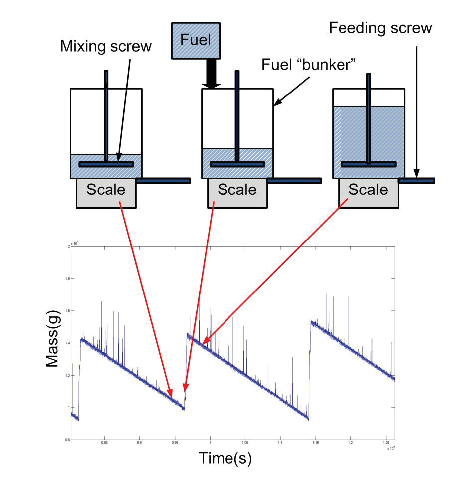
\includegraphics[width=0.45\textwidth]{pics/cfb_paper/OMF/MassFlowScheme}
\caption{The origin of the input signal ~\cite{ZliobaiteBP09}.}\label{fig:OMF}
\end{figure}

In the previous work~\cite{ZliobaiteBP09,BakkerSensorsKDD09,DBLP:conf/incdm/IvannikovPBLJKA09} outliers were removed,
burning and feeding stages were detected and mass flow was estimated with a high accuracy. The main results were summarized in~\cite{PechenizkiySIGKDDExpl09}.
However, occasional gradual changes in the signal caused by increasing or decreasing frequency of the mixing screw have not been addressed.
This is the problem that we focus on for this case.

\section{CHANGE DETECTION METHODS}
\label{sec:ourapproach}

There are many methods applicable to the problems we consider. We discuss here the density-ratio estimation and control charts which are fundamental for our domain and then present our Quantile Index (QI) approach.

\subsection{Density-Ratio Estimation}
The basic concept underlying the statistical change detection algorithms is the
logarithm of the likelihood ratio, defined by 
\begin{equation} \label{eq:lr1}
s(y) = ln \frac{p_{\theta_{1}}(y)}{p_{\theta_{2}}(y)}.
\end{equation}
% \subsection{Likelihood Ratio}
The likelihood of a sample is the probability of obtaining that particular sample,
given the chosen probability distribution model. This expression contains the unknown model parameters.
The values of these parameters that maximize the sample likelihood are known as the
Maximum Likelihood Estimates. 
A change in the parameter $\theta$ in (\ref{eq:lr1}) is reflected as a change in the
sign of the mean value of the log-likelihood ratio \cite{I.V.Nikiforov}.

But this approach is affordable in case if at least the parameter $\theta_{0}$ before the change is known.
In this case hypothesis testing between two hypotheses $H_{0}: \theta = \theta_{0}, H_{1}: \theta = \theta_{1}$
should be performed in an on-line manner by means of the decision function:
\begin{equation}\label{eq:lr2}
S_{j}^{k} = \sum_{i=j}^{k}  ln \frac{p_{\theta_{1}}(y_{i})}{p_{\theta_{2}}(y_{i})}.
\end{equation}
This is the underlying concept for control charts that we consider next.

\subsection{Shewhart control charts}

Statistical properties of the data can be marked on the graph by drawing an Upper/Lower Control Limits (UCL and LCL) for the selected feature $\theta$.
Control limits are two lines which indicate the state of the `in control' process.
It means that data points lie within those limits with a high predefined probability.
Strictly speaking we cannot use the term probability because we do not know a statistical distribution of the data.
But we can use a fraction of out-of-control points as an indicator of the state.
There is a probability that some points will fall outside the limits even if no actual change of feature $\theta$ has happened. 
The process can be described by the following three values:
\[ UCL = \mu_{w} + k\sigma_{w},\] \[Center Line = \mu_{w},\] \[  LCL = \mu_{w} - k\sigma_{w}. \]
The main object of interest is a set of rules defining when to update control limits.

The $CenterLine$ of the process and \textbf{$\sigma$} are unknown in general.
We just can estimate them from the set of sampled examples given some statistical assumptions. 
The standard deviation of the sample 
\[s = \sqrt{\frac{\sum_{k=1}^n (x_{i} - \overline{x})^2}{n-1}} \]
is just an estimator of the unknown standard deviation $\sigma$ of the data from which it is being sampled.
If the underlying distribution is known, e.g.\ normal, the corresponding parameters can be easily estimated~\cite{Nist}.

In manufacturing processes an action should be taken even if one point falls outside limits.
Due to specificity of our data we can determine a priori a threshold of the fraction of points which fall outside limits.
It changes over time and we have to deal with a streaming data which we have to treat on-line.
By monitoring the amount of points that fall outside control limits we can decide about the change and model update to be performed.

To keep the discussion compact we do not consider CUSUM control charts~\cite{cusum}.

\subsection{Quantile Index Method}
If we apply control charts we need to know the value of a statistical parameter, which changes over time, before the change.
Quantile Index (QI) is even a simpler approach and effectively is parameter free. 

Quantiles are points taken at regular intervals from the empirical cumulative distribution function that mark the boundaries between the consecutive subsets
(Figure~\ref{fig:PDD_quantile}).

\begin{figure}[htb!]
\centering
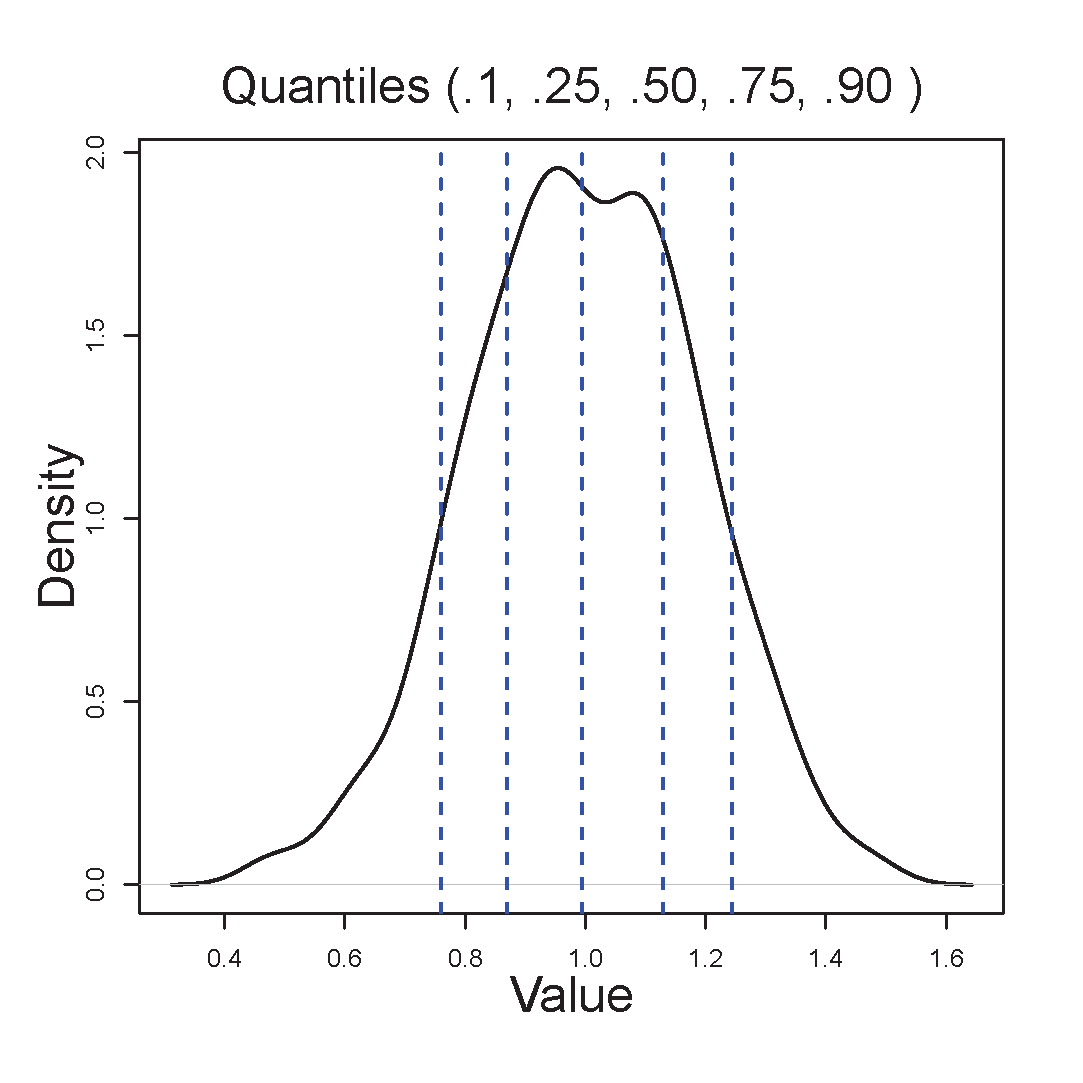
\includegraphics[width=0.4\textwidth]{pics/cfb_paper/QuantileDef}
\caption{The probability density distribution illustrating quantile values: $10\%$ of all points have values less than 0.76 (the first dashed line),
$15\%$ of all points lie between the first and the second dashed lines (because there are quantiles with probabilities $10\%$ and $25\%$), etc.}
\label{fig:PDD_quantile}
\end{figure}

We consider two basic cases: an increase in the mean and an increase in the variance of a signal. 
As an indicator of a state we keep track of the top boundary of the data points by moving quantiles with maximum probability. 
When a change has happened we observe a kind of step function. By selecting an appropriate width of a sliding window we make this track line insensitive to outliers; but it allows us to detect steady changes.
For this purpose we use two quantiles with probabilities $90\%$ and $100\%$.
The intuition is that after a change there is no intersection between the data points falling in between the current $90-100\%$ quantiles and between the same quantiles in the past. Therefore QI will demonstrate a sharp change even in the case of a gradual change in the signal.

The change detection method based on QI works as follows:
\textit{
At each moment of time we consider a range of data which is divided into two subsets corresponding to the Test Interval and the Reference Interval.
We compute the minimum Index of observations in the Reference window which values are in the range between quantiles of the measurements in a Test window} (Figure~\ref{fig:QI_scheme}).

\begin{figure}[htb!]
\centering{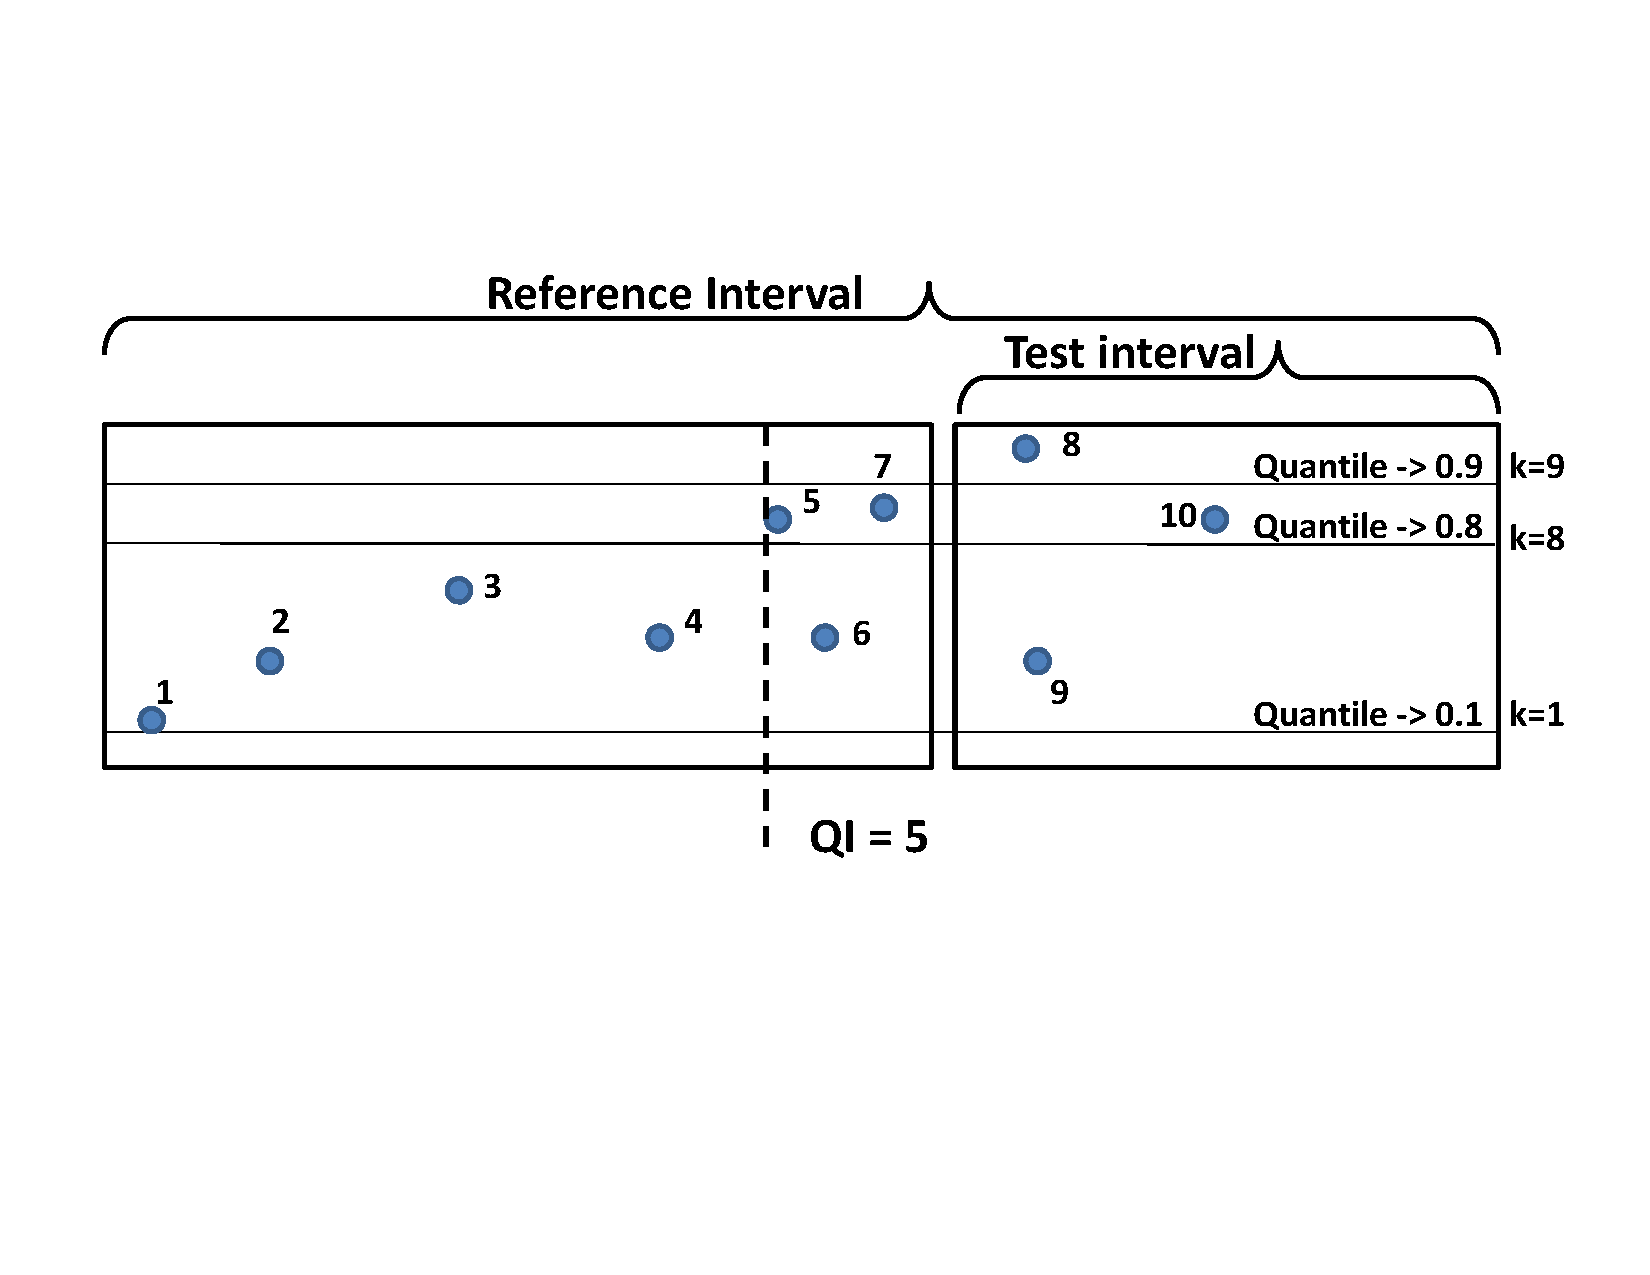
\includegraphics[width=0.45\textwidth]{pics/cfb_paper/QIdefinition}}\\
\caption{QI method illustration. %Beginning of the \emph{reference interval} should start from the last detected change or from the beginning of a signal if there has been no change detected so far.
QI depicts the position of a point with the smallest index which lies between quantile 0.9 limits
in the Test interval.}
\label{fig:QI_scheme}
\end{figure}

Thereby we determine a `similarity' between chunks of the data.
Quantiles are computed from the inverse of the empirical distribution function.
In other words, the $p$'th quantile of $X(0<p<1)$ is defined by:
\[
Q_{p}=F_{X}^{-1}(p).
\]
Given the probability $p$ and sorted data vector $x$, quantile estimation could be calculated as follows:
\[
Q(p) = (1-\gamma)x[j] + \gamma x[j+1],
\]
where $j=floor(np)$, $n$ is the sample size, $\gamma = 0$ if $p=0$, and $1$ otherwise \cite{Rref}.
There are two ways for calculating statistics on-line.
One approach is to calculate it over a sliding window at each moment of time. %(Short QI).
The second way is to calculate cumulative statistics from the beginning up to the current moment.
It is more robust but also more computationally expensive.
We compute QI for both cases by means of different sizes of a sliding window.
The pseudocode for computing cumulative QI for the current Reference and Test Intervals is presented below:
\begin{verbatim}
w - window width; 
i - data point sliding index;
Q - array to store quantiles;
k = 10 - index determining quantiles to be used;
QI - quantile index returned as an output;

Reference Interval <- data[1:i]
Test Interval <- data[(i-w+1):i]
# array of probabilities:
Probability  <- {0.1,...,0.9,1}
Q <- quantile(Test Interval, Probability)
QI <- which((Reference Interval >  Q(k-1)) and
            (Reference Interval <= Q(k)))
QI <- minimum(QI)
\end{verbatim}

Function \textit{which()} returns indexes of data points which satisfy condition in brackets. For the example in Figure~\ref{fig:QI_scheme}, \textit{which()} will return $\{5,7,10\}$ and consequently, $QI=5$.
These calculations should be performed for each time step over a sliding test interval.

\section{Experimental study}
\label{sec:experiments}
First, we show the behavior of QI on the artificial data. 
We show explicitly values of $90\%$ and $100\%$ moving quantile values by which QI is being determined and the sensibility of QI to perturbations in the signal which affect quantiles online estimation.
Then, we evaluate the performance of QI and other considered approaches on two real datasets.

\subsection{Artificial Data}
We compute QI values for generated data with known statistical properties in order to
demonstrate behavior of QI depending on the test interval width.
There are three blocks of samples from uniform distribution each length of 1000 with a range width equal to 1 (Figure~\ref{fig:figure3.0}).
Each block is shifted by the $step = 0.15$ relative to the previous one.
The artificial data is produced in a similar way as described in ~\cite{journals/tkde/TakeuchiY06,Kawahara_2009}.

\begin{figure}[htb!]
\centering{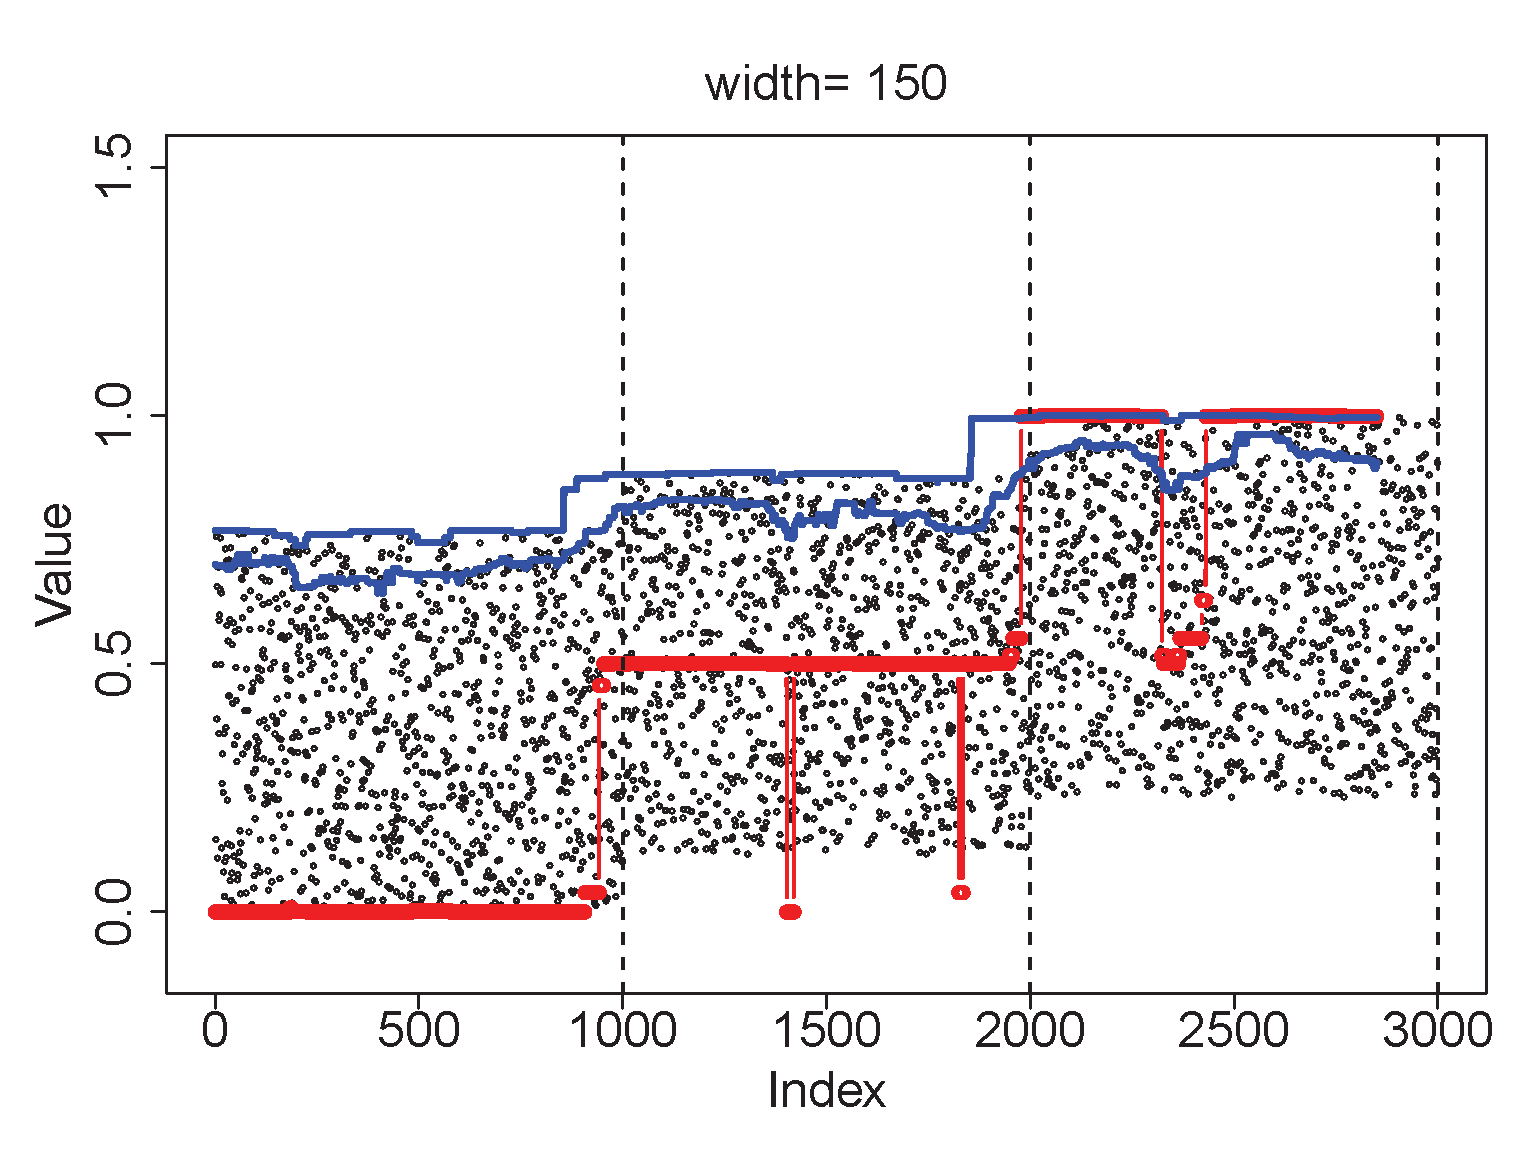
\includegraphics[width=0.45\textwidth]{pics/cfb_paper/DebugDataSet/DataPIC150}}\\
\centering{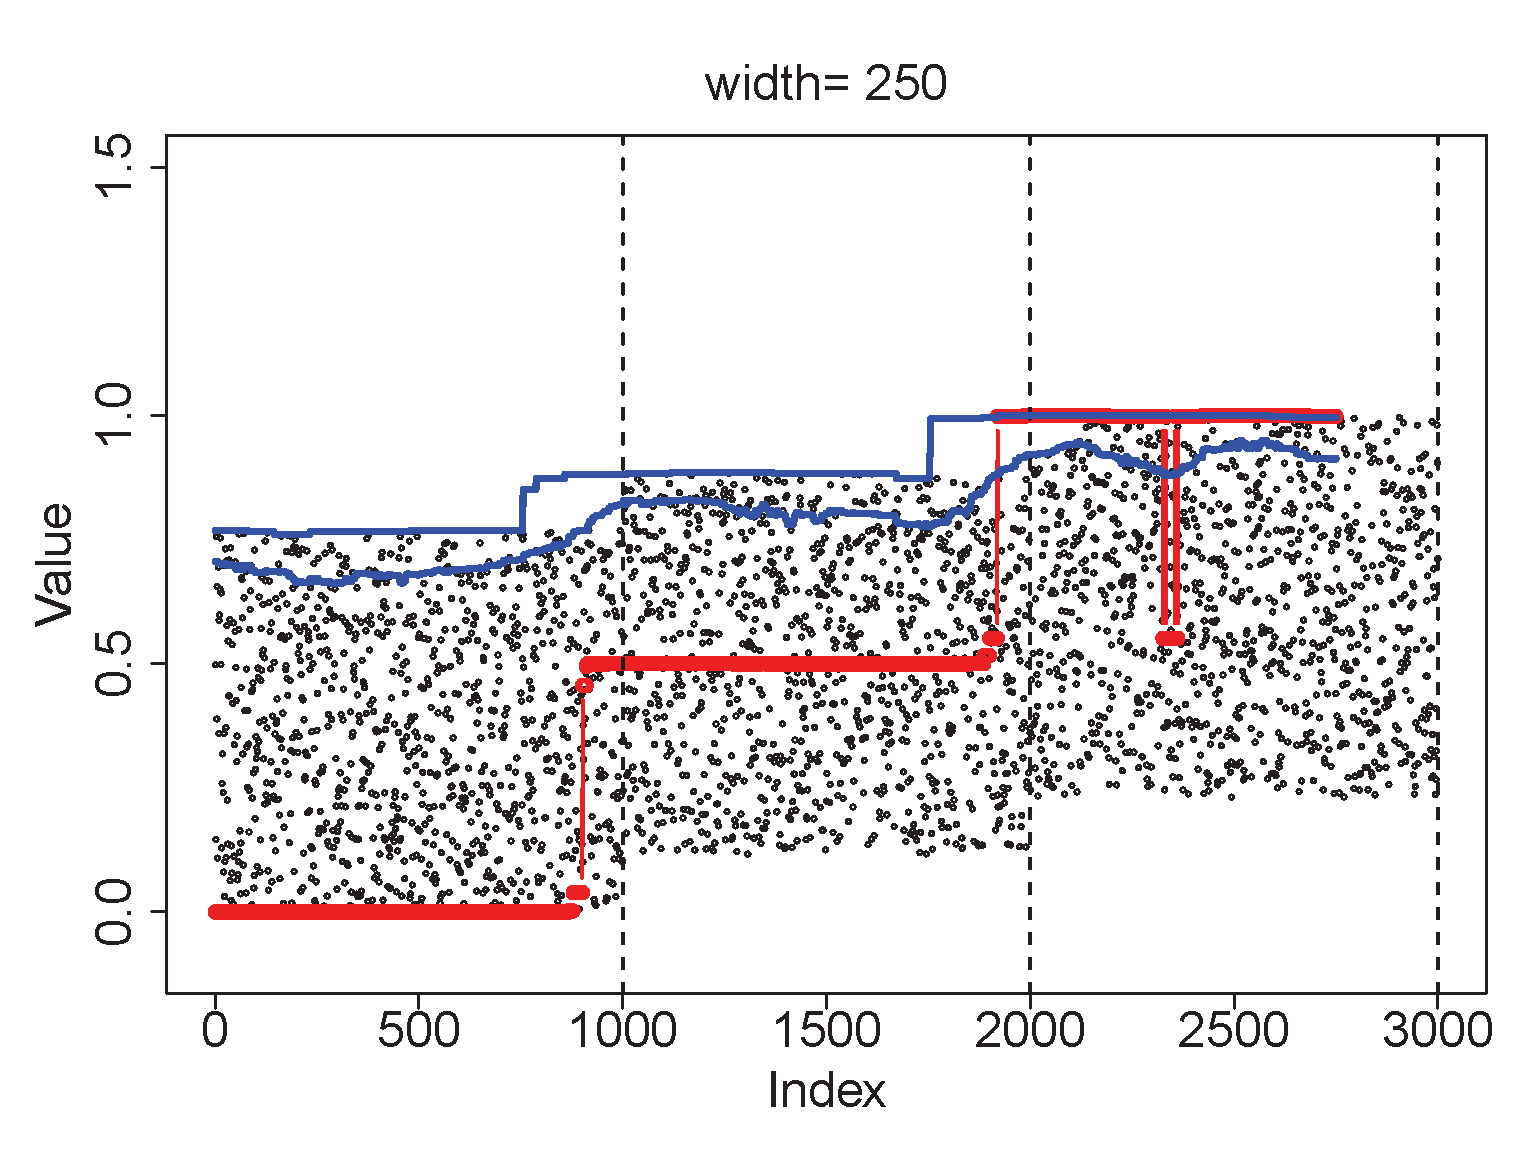
\includegraphics[width=0.45\textwidth]{pics/cfb_paper/DebugDataSet/DataPIC250}}
\caption{Behaviour of scaled QI values (red dots), quantiles values (blue dots) for uniformly distributed data (black dots).}
\label{fig:figure3.0}
\end{figure}

\begin{table}[htb!]
%\centering
\caption{Performance of QI on the artificial data. The bigger the test interval the more robust to quantiles values fluctuations QI is.}
\begin{tabular}{|l|l|l|l|l|l|l|}
\hline
	Test Interval width            & 50  & 70  & 90  & 120 & 130 & 150 \\ \hline
	False alarm rate & 19  & 10  & 8   & 6   & 6   & 5   \\ \hline
	Test Interval width			 & 170 & 190 & 210 & 230 & 250 &     \\ \hline
	False alarm rate & 4   & 3   & 2   & 1   & 1   &     \\
\hline
\end{tabular}
\label{Table1}
\end{table}

\subsection{Pressure fluctuation change}

The dataset comes from the controlled experiment in the laboratory settings. The sensor was measuring the dynamic gas pressure in the cold model CFB system.

The dataset consists of 3 800 001 data points (the sampling rate dt(s): 5000 Hz) corresponding to the duration of 12 minutes and 40 seconds.
%The measurements were taken with high frequency.
We consider down sampled signal for the computational and visualization convenience.
The sample frequency 20 Hz for pressure fluctuations can be considered as a lower limit.
But typically, a sample frequency in the order of 200-400 Hz is applied ~\cite{vanOmmen2011403}.

At a particular moment, particles with another average size were added inside a container.
It caused abrupt change in the signal (Figure~\ref{fig:psd_change}, $t=223$). Further mixing of particles is manifested by the gradual change in the amplitude of pressure. The signal is symmetrical because we use the first difference of the original signal.

\begin{figure}[htb!]
\centering{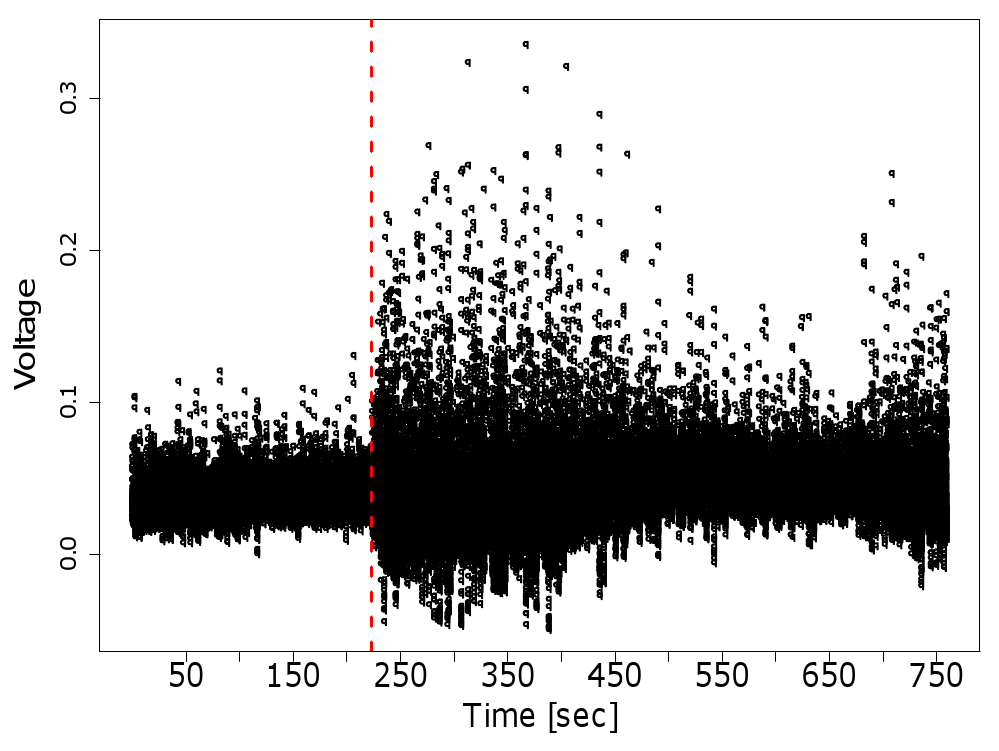
\includegraphics[width=0.45\textwidth]{pics/cfb_paper/PSD/PSDsampled}}
\caption{Adding of particles with another PSD.}\label{fig:psd_change}
\end{figure}

Figure~\ref{figure7} shows the Box-And-Whisker diagram, in which each box represents 5 values: the largest and smallest values, median, and the highest and lowest quartiles. From the diagram we can see more explicitly the gradual change near the 16th-17th data windows.

\begin{figure}[htb!]
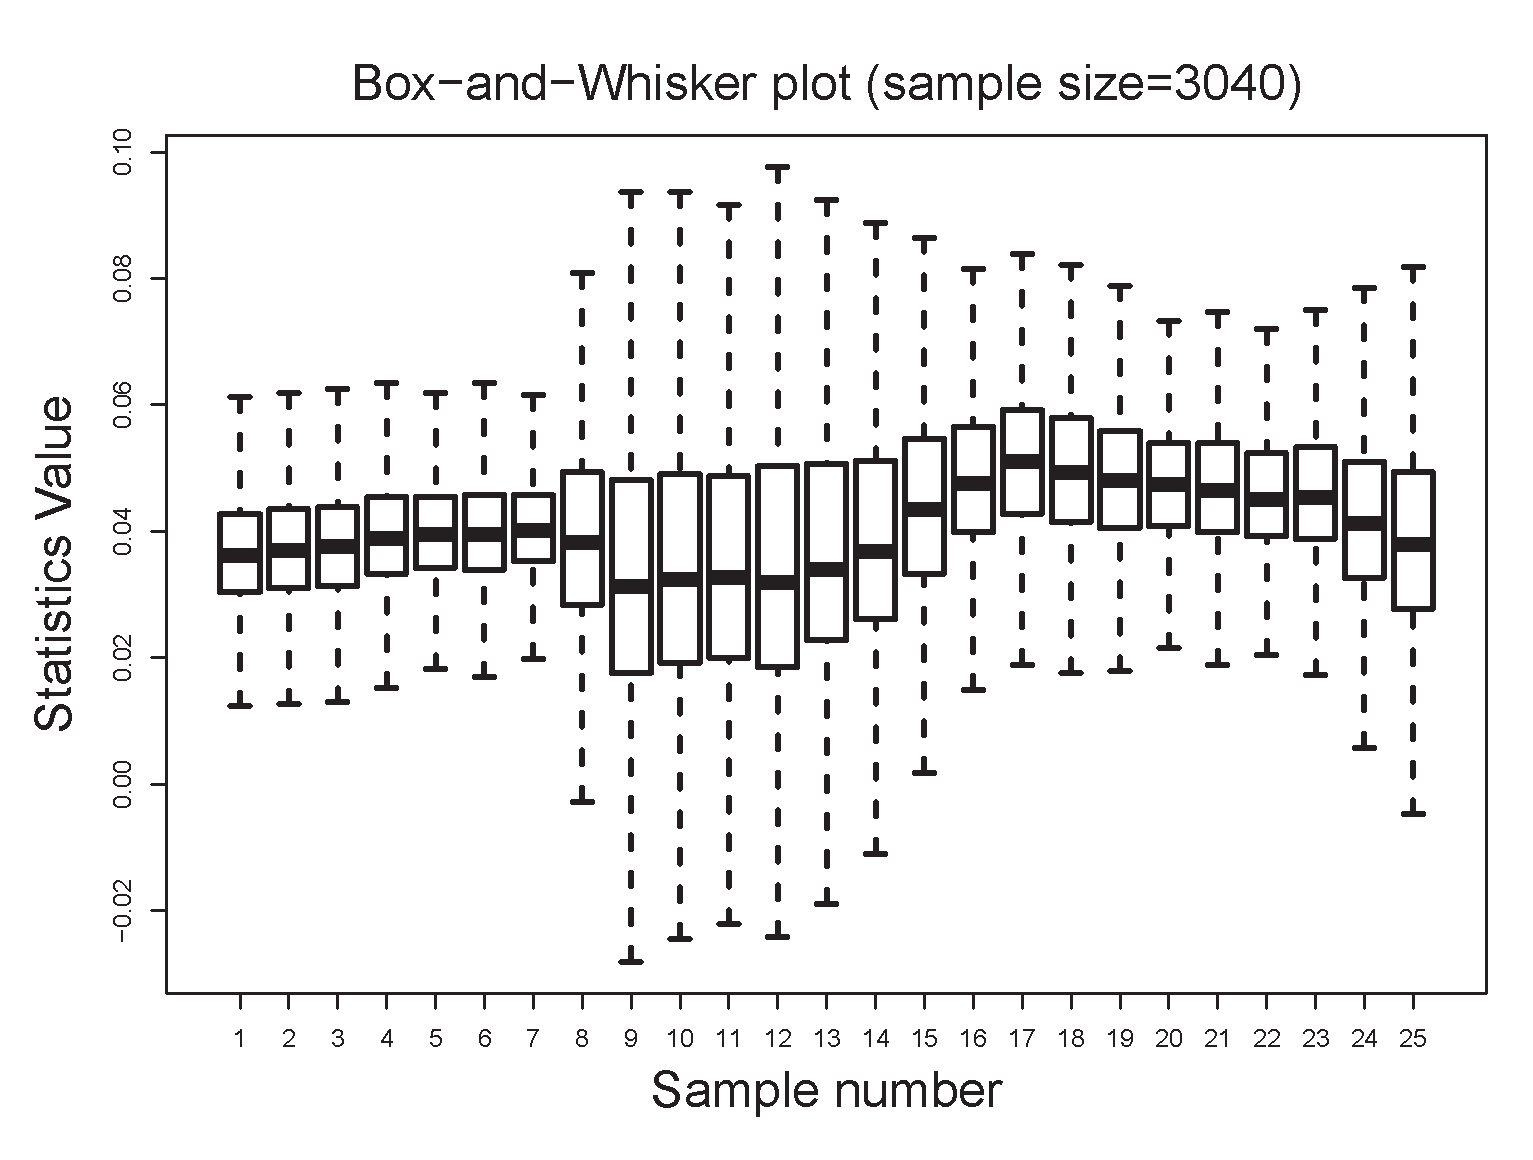
\includegraphics[width=0.45\textwidth]{pics/cfb_paper/PSD/PSDboxplot}
\caption{Box Plot for sampled signal. Signal was divided into groups of samples. Each box
on the graph represents 5 statistics for each group.}\label{figure7}
\end{figure}

Figure~\ref{figure8} shows the probability density estimations of the data before and after change. We can see that the averages are almost the same, but the standard deviation values are quite different.

\begin{figure}[htb!]
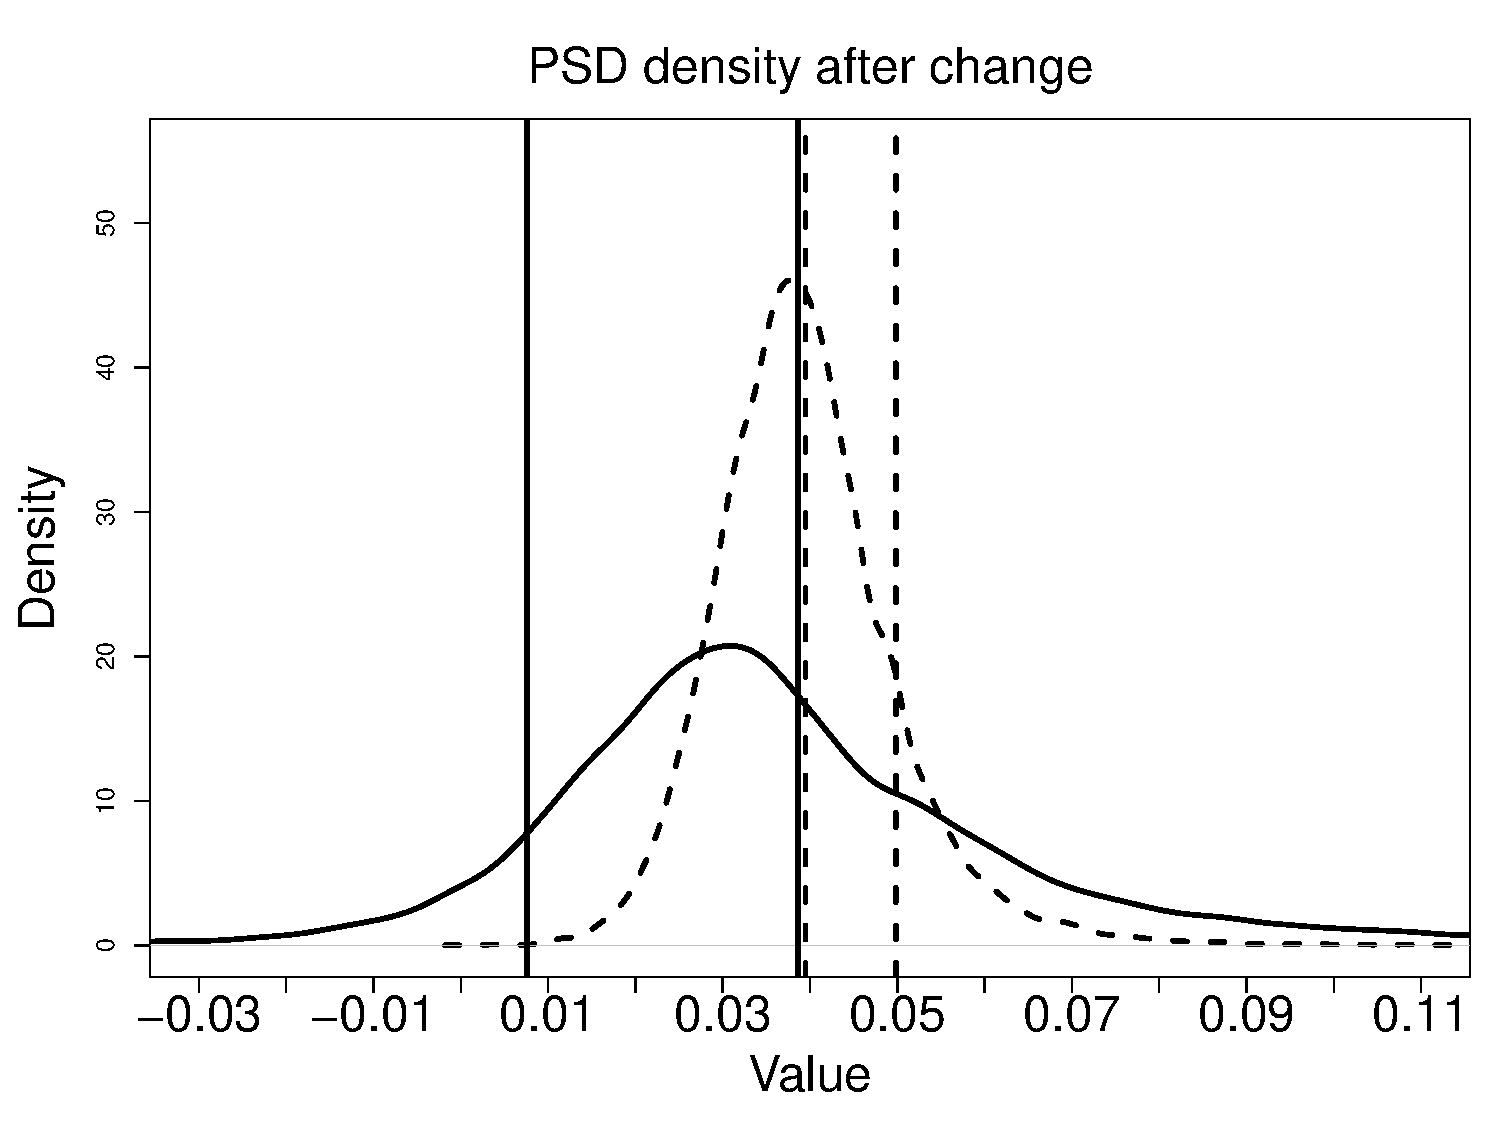
\includegraphics[width=0.45\textwidth]{pics/cfb_paper/PSD/PSDdensity}
\caption{Estimation of a probability density of a signal before and after change.}\label{figure8}
\end{figure}

From Figure~\ref{figure9} we can see that the most significant change happened in the standard deviation and the range of values:
$(Mean2 - Mean1)/Mean1 = 0.02$, $(Std2 - Std1)/Std1 = 1.99$. The first 250 seconds time range is considered as process in control, because we know that no particles have been added by this moment and some time after. Accordingly to the standard rules, the process in control points should fall within $3\sigma$ limits. 

\begin{figure}[htb!]
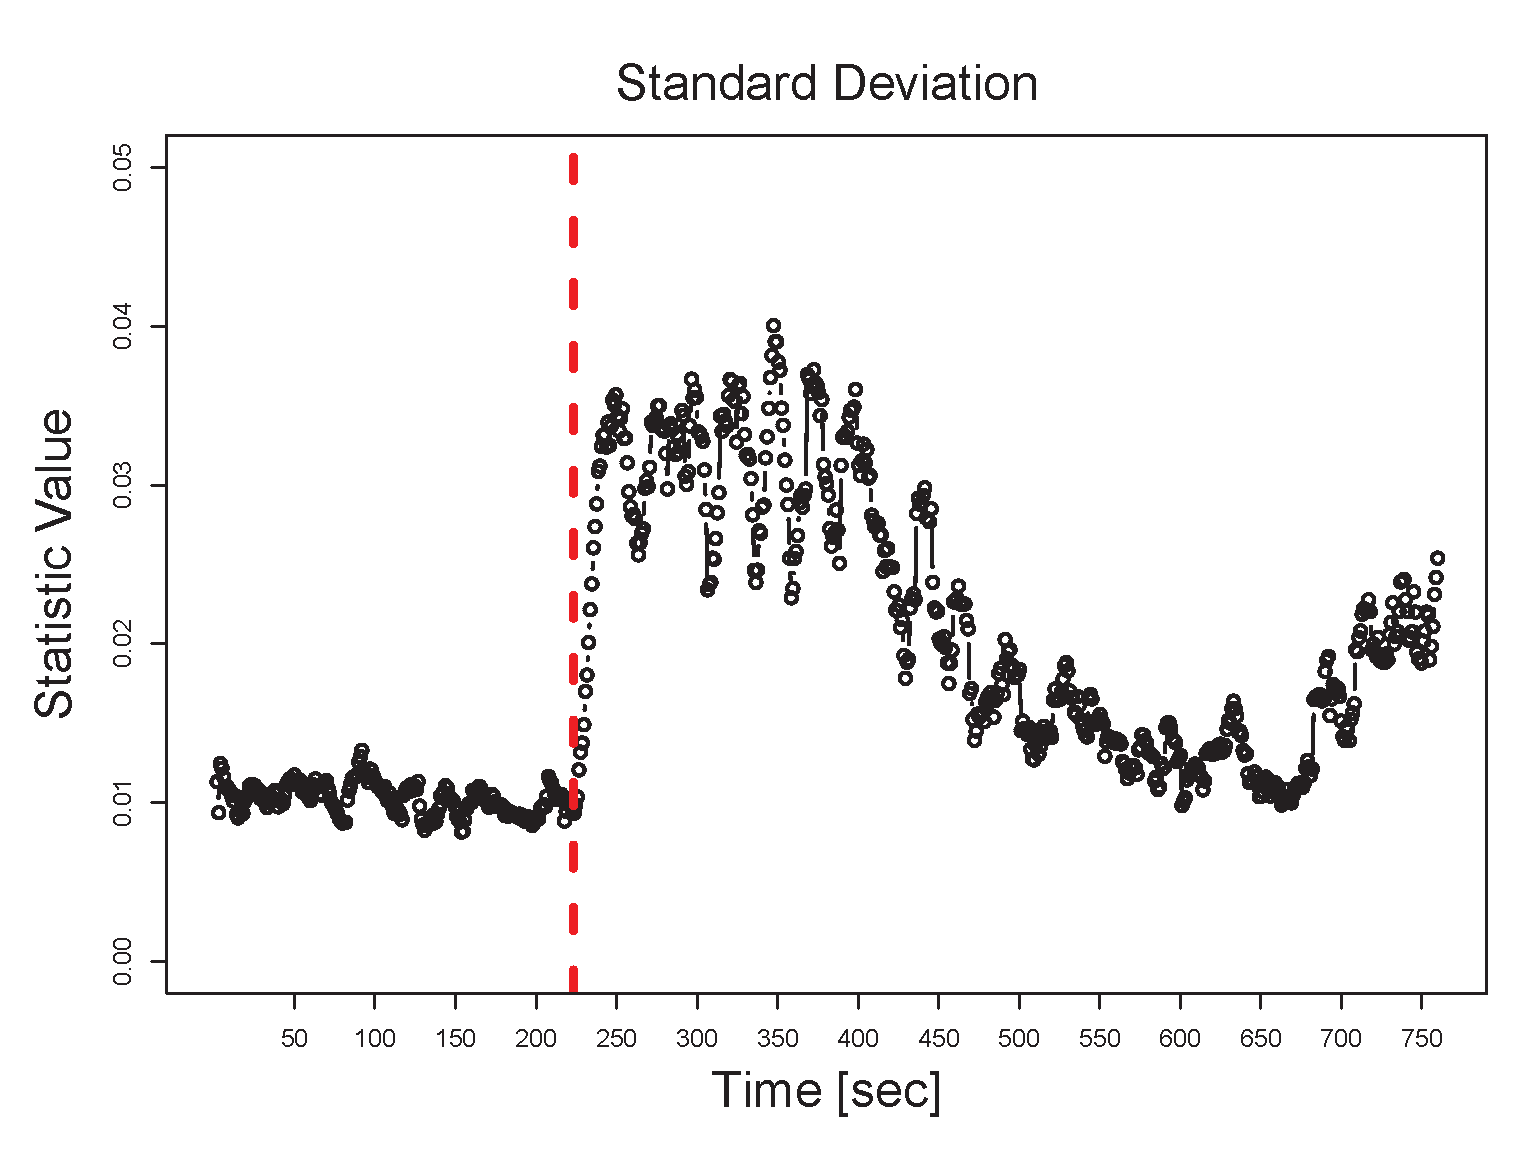
\includegraphics[width=0.45\textwidth]{pics/cfb_paper/PSD/PSDsd}
\caption{Moving standard deviation -- a promising feature to use for change detection.}\label{figure9}
\end{figure}

\paragraph{Change detection with Control charts for moving SD}
We consider the first difference of the moving standard deviation.
We define new control limits for a process each time when we have more than $10\%$ points beyond control limits and
when current control limits are greater more than 1.5 times than $3\sigma$ (Figure~\ref{figure10}).

\begin{figure}[htb!]
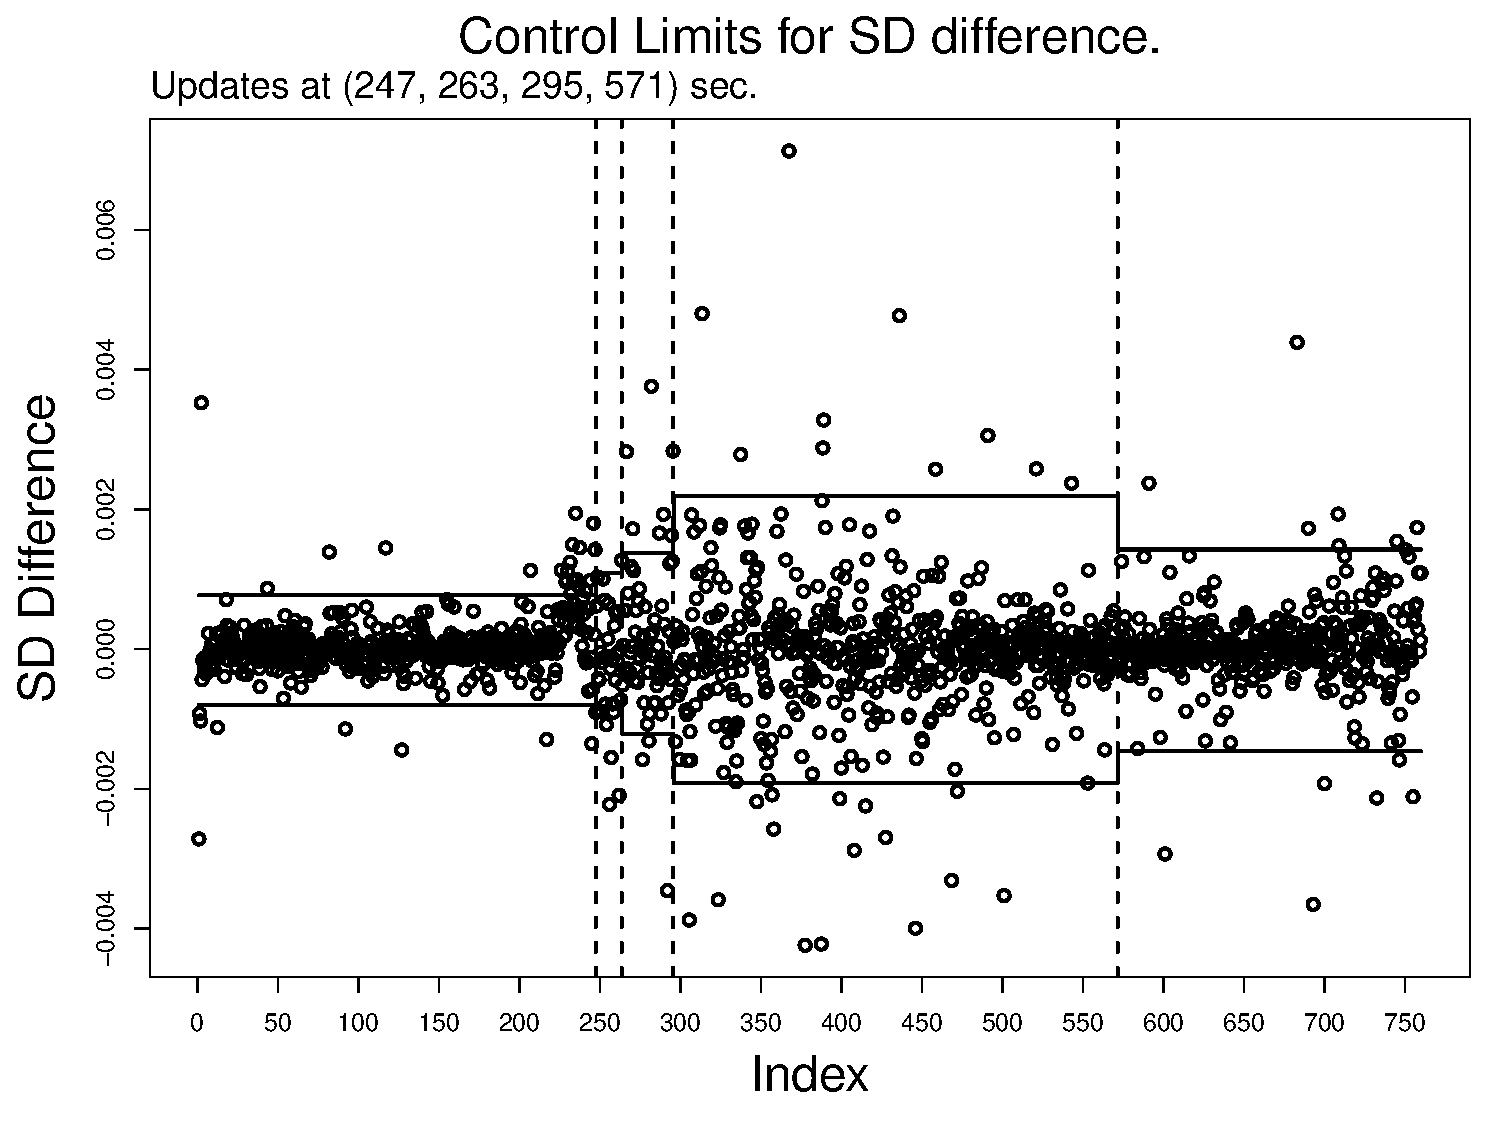
\includegraphics[width=0.45\textwidth]{pics/cfb_paper/PSD/PSDrunnqccSD}
\caption{Control charts for the first order difference of the moving standard deviation.
New control limits are updated each time when more than $10\%$ of points fall beyond limits.}\label{figure10}
\end{figure}

Updates were performed four times: $t=\{247, 263, 295, 571\}$. 
The latency of the detection is $(247-223)=24$ seconds.

\paragraph{Detection with Quantile Index}
%Let's apply QI for the same data.
We can use different features in order to apply control charts.
But which one is the most sensitive to the abrupt changes and for gradual changes?
QI is robust to outliers and noise presence; therefore we can apply it directly to the raw data.
We detect a change in case of significant increasing of QI values relatively to the previous QI.
The criterion we us is 
\begin{equation}\label{QIcriterion}
log \frac {QI[i]}{QI[i-1]} \geq threshold.
\end{equation}
%$log(QI[i]/QI[i-1]) >= threshold$.
Change points detected with QI are shown in Figure~\ref{figure12}. The latency of the detection for the known change at $t=248$ is $(248-223)=25$ seconds.

\begin{figure}[htb!]
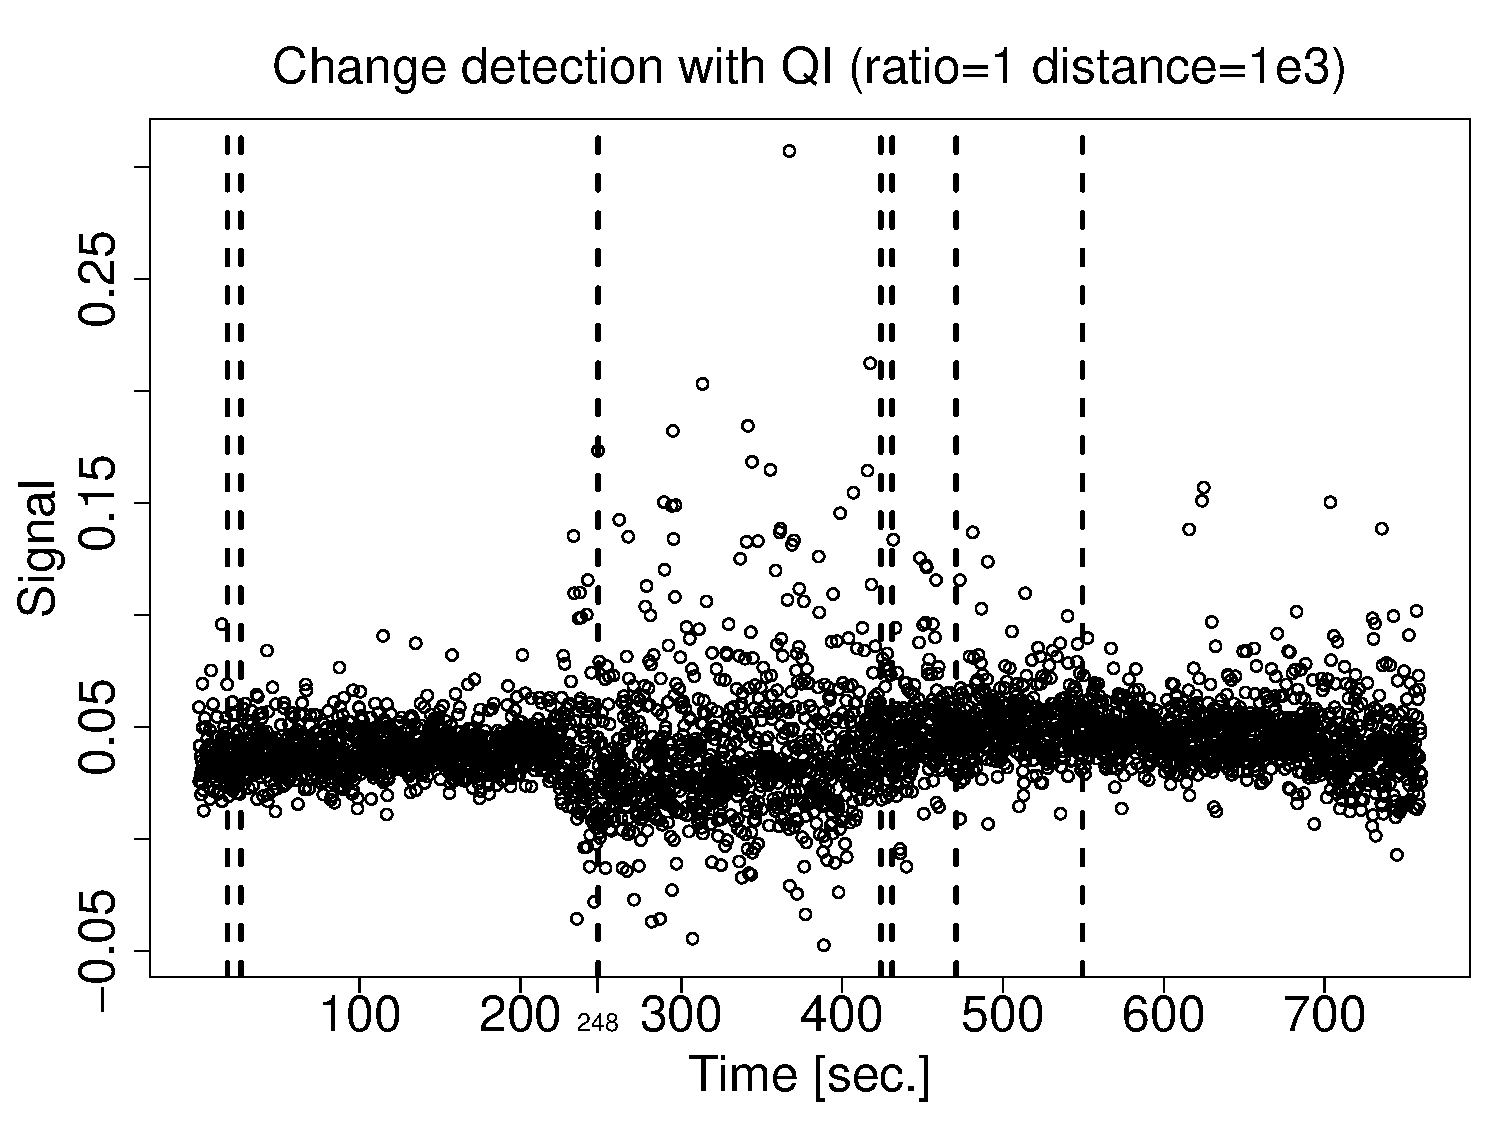
\includegraphics[width=0.45\textwidth]{pics/cfb_paper/PSD/PSDsteadyQI1}
\caption{Change detection with QI on raw data.}\label{figure12}
\end{figure}

\paragraph{Detection with Density Ratio Estimation}

Modifying eq.~\ref{eq:lr2} to our reference and test intervals we get
\begin{equation}\label{KDEformula}
S = \sum_{i=1}^{n_{te}}  ln \frac{p_{te}(Y_{te}(i))}{p_{rf}(Y_{te}(i))},
\end{equation}
where
\begin{equation}
w(Y)=\frac{p_{te}(Y_{te}(i))}{p_{rf}(Y_{te}(i))}
\end{equation}
is the density ratio.

Further we conclude
\begin{equation}
\begin{cases}
S \leq \mu \rightarrow \phantom{1} no \phantom{1} change \phantom{1} occurs, \\
otherwise  \rightarrow \phantom{1} a \phantom{1} change \phantom{1} occurs,
\end{cases}
\end{equation}
where $\mu >0$ is a predetermined threshold~\cite{Kawahara_2009}.

Figure~\ref{figure12.1} shows change detection results with the online non-parametric Kernel Density Ratio estimation (KDE) algorithm.
\begin{figure}[htb!]
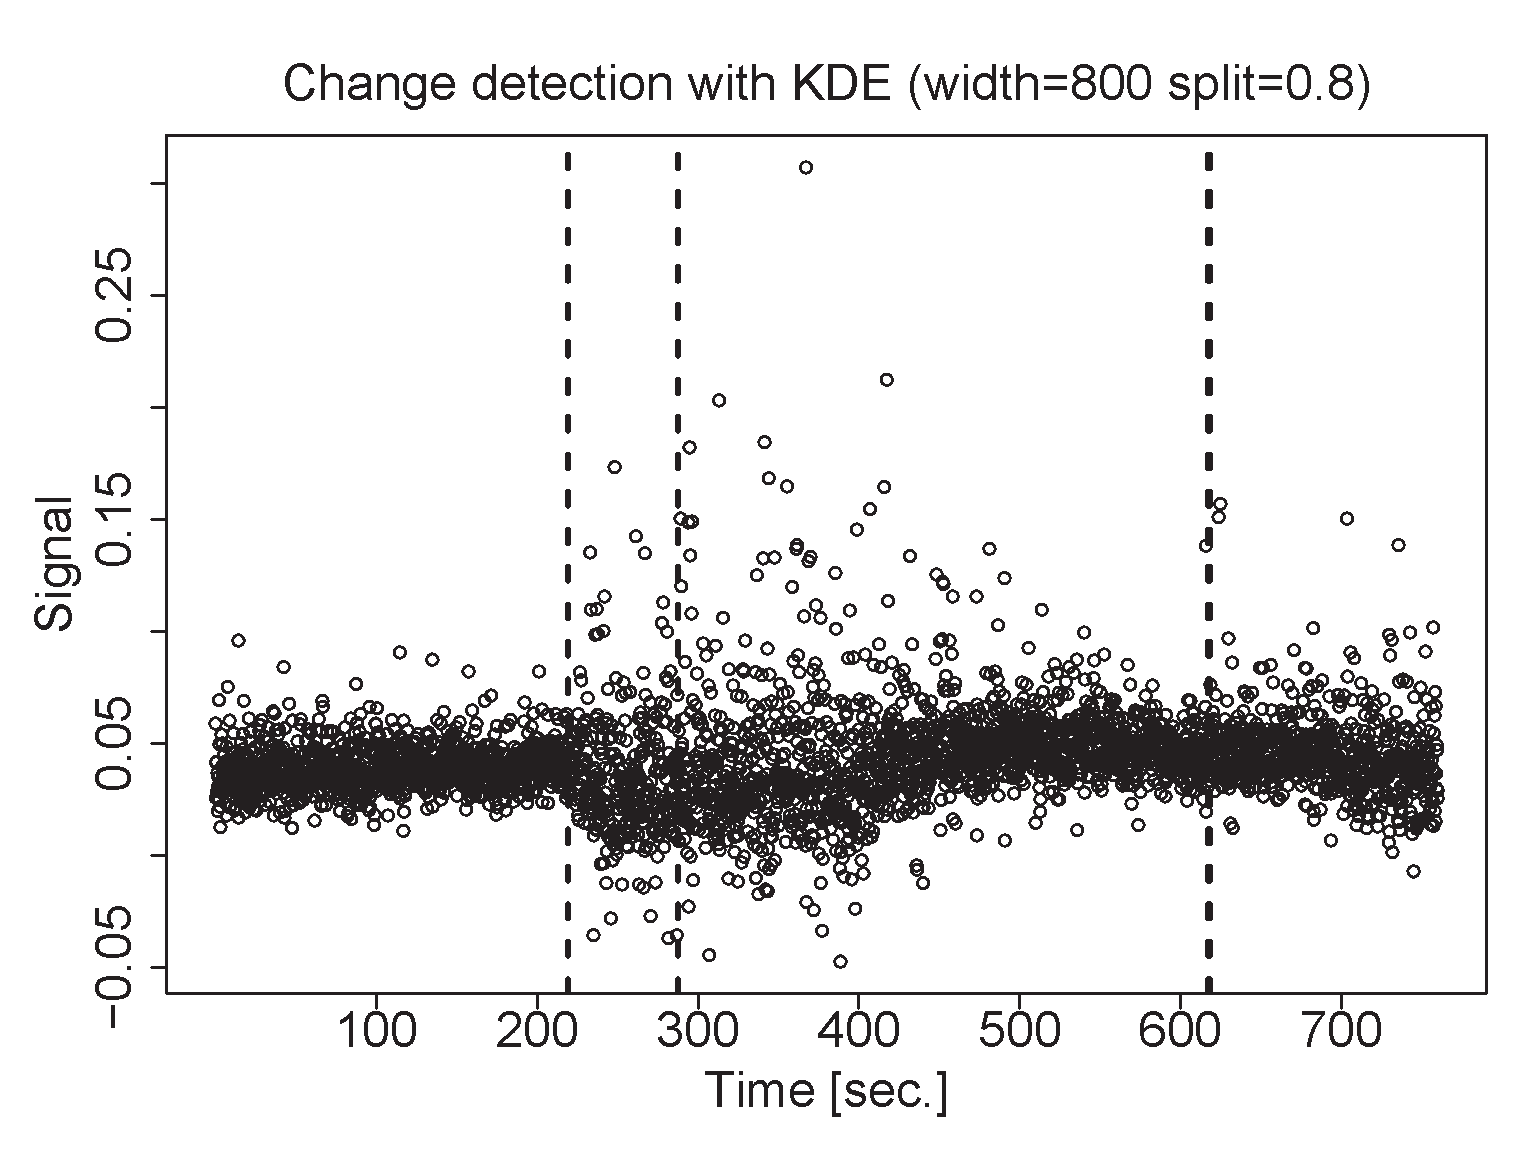
\includegraphics[width=0.45\textwidth]{pics/cfb_paper/PSD/PSDkde}
\caption{Change detection with KDE. Detected points: $t=\{219,274,614\}$.}
\label{figure12.1}
\end{figure}

\subsection{Mass Flow Signal}

The signal has the following properties. It reflects burning and feeding stages (both are abrupt changes).
The signal itself is noisy due to the disturbances of the physical system that vibrates and shakes from time to time when particles are jammed with the mixing screw.
Besides, there is a room for gradual change due to change in the mixing screw frequency.
Although the change in the signal is gradual, it was caused by abrupt change in the frequency -- see Figure~\ref{figure15} for the illustration.
We should notice that there are a lot of not only noise but outliers too that
makes change detection and especially gradual change detection rather challenging.
Figure~\ref{figure18} shows the both the abrupt and the gradual changes.

\begin{figure}[htb!]
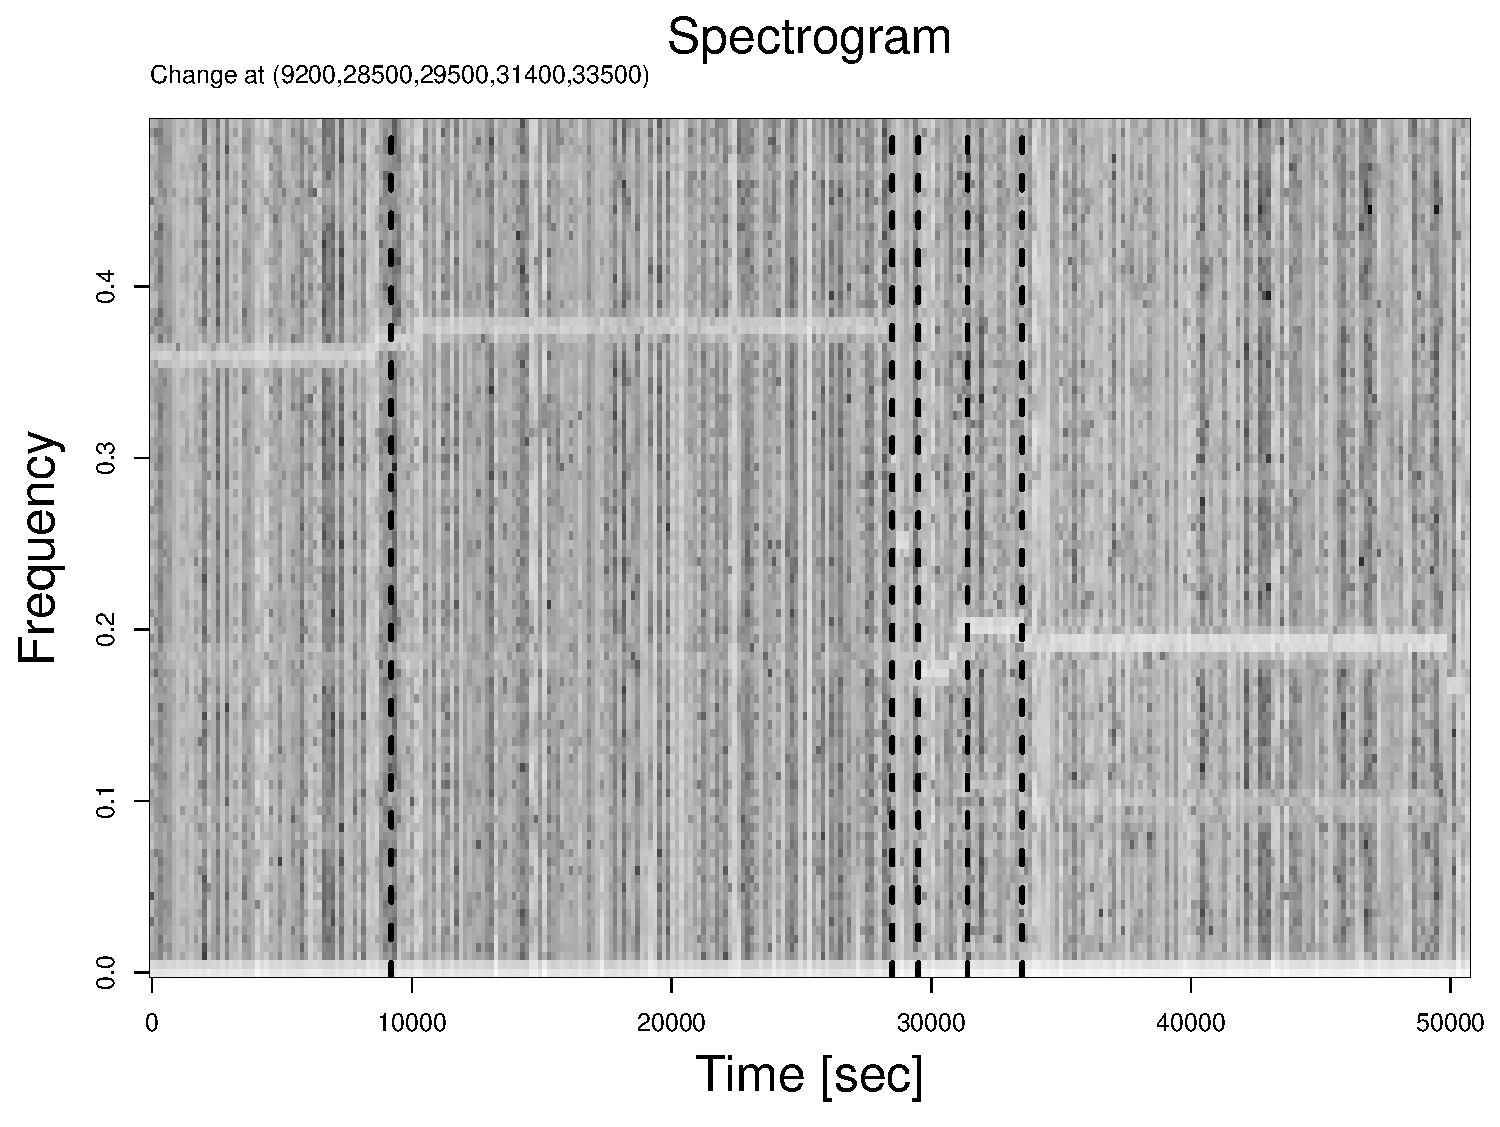
\includegraphics[width=0.45\textwidth]{pics/cfb_paper/OMF/OMFspg}
\caption{Spectrogram showing frequency changes.}\label{figure15}
\end{figure}

As a fuel mass estimation we use the sequence of points at the bottom of a signal, or, in other words, the lowest quantile at each moment of time (Figure~\ref{figure16}).

\begin{figure}[htb!]
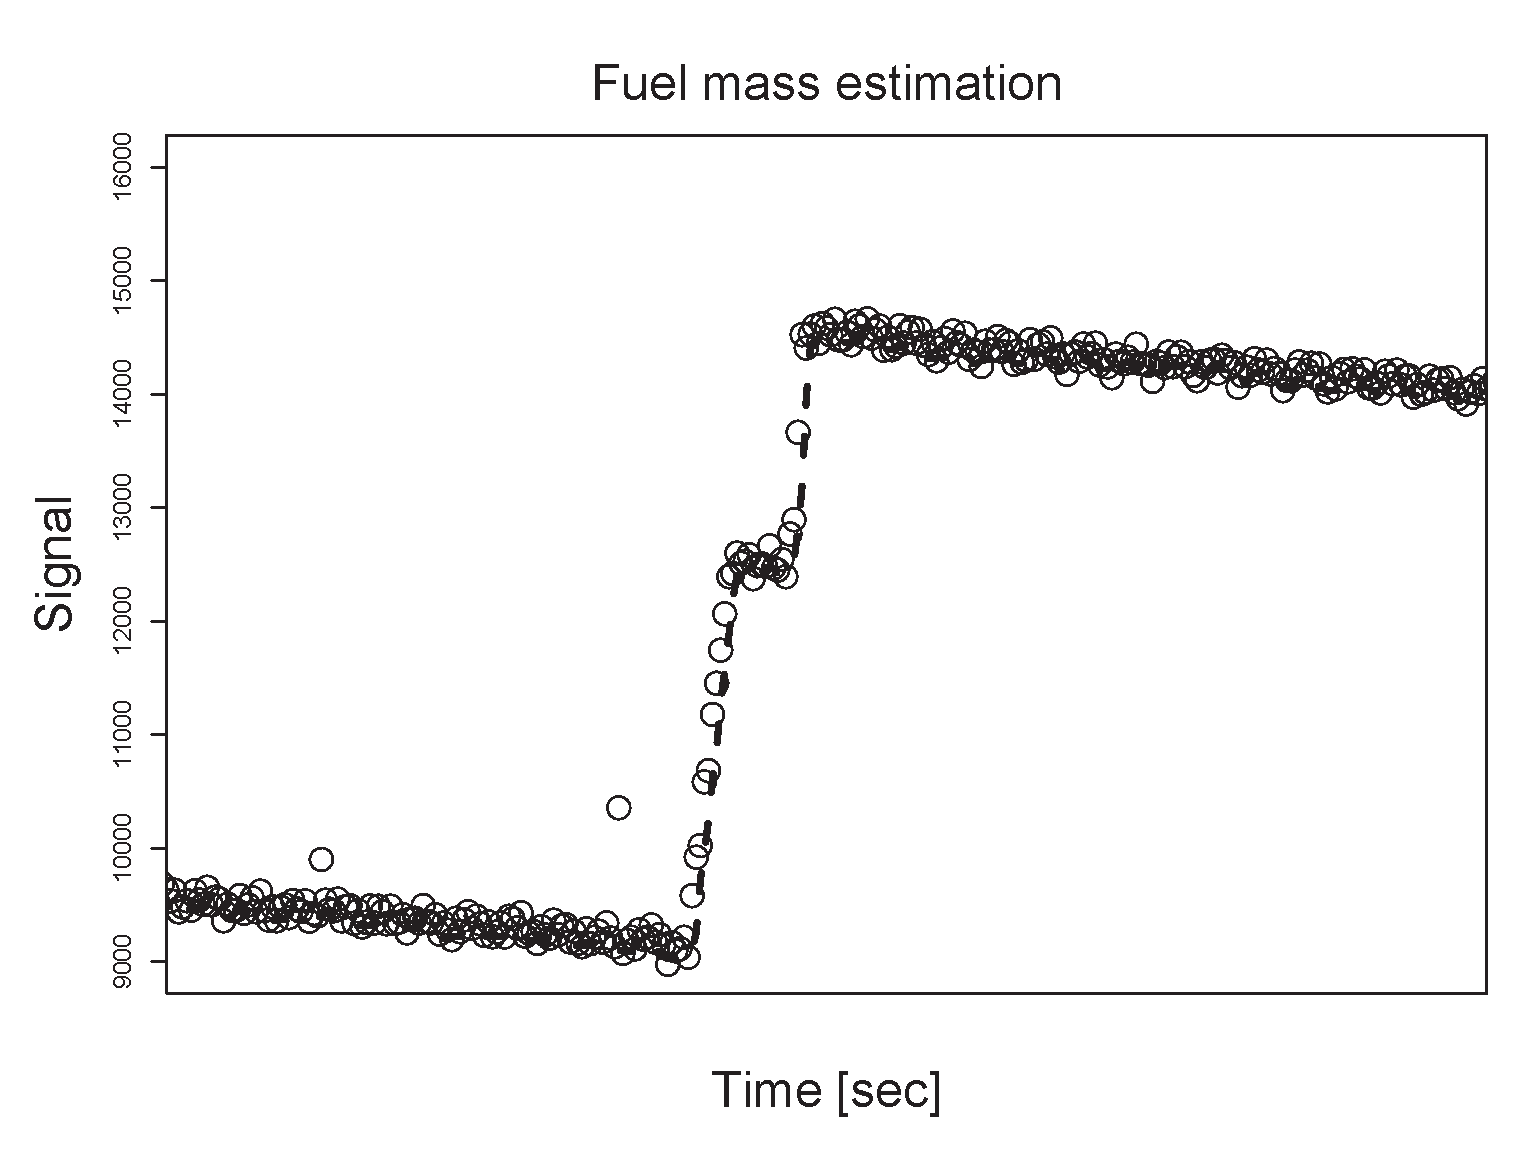
\includegraphics[width=0.45\textwidth]{pics/cfb_paper/OMF/OMFestim2}
\caption{Fuel mass estimation using $5\%$ quantile (dashed line) computed over the sliding window.}\label{figure16}
\end{figure}

\begin{figure}[htb!]
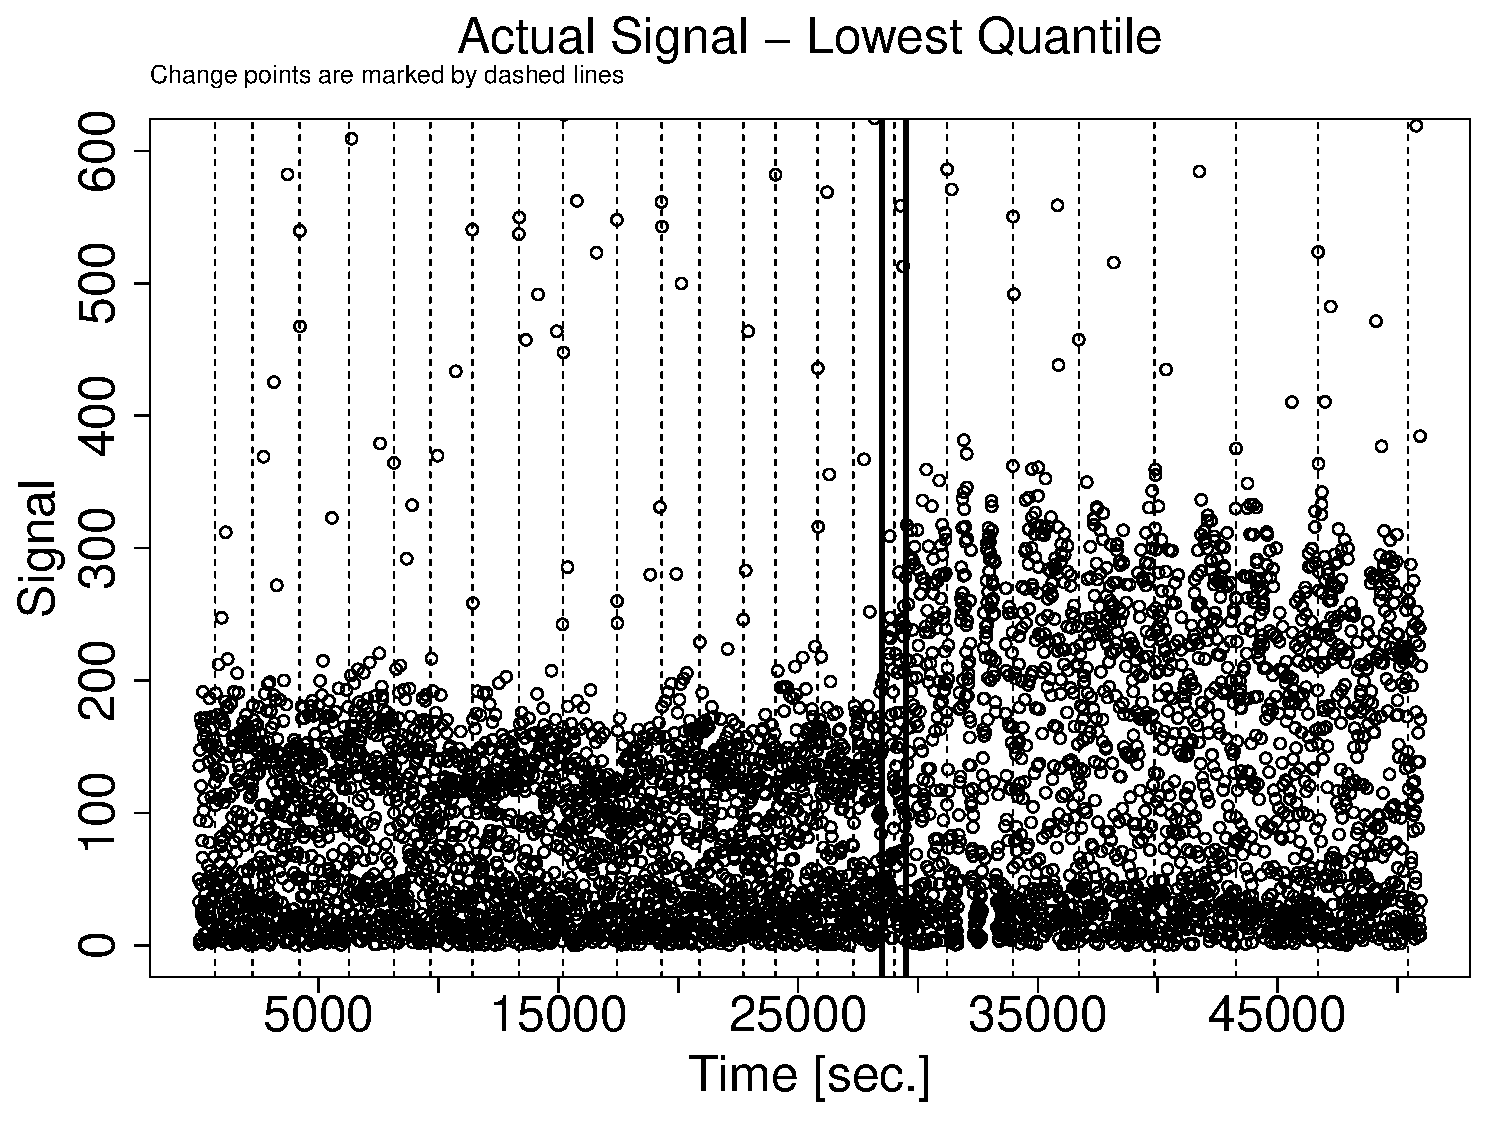
\includegraphics[width=0.45\textwidth]{pics/cfb_paper/OMF/OMFscalednoise}
\caption{Mass flow signal with marked change points, determined by visual inspection of the original signal and the spectrogram.
There are a lot of changes due to switching between burning and feeding stages (depicted by thin dashed lines) and
two changes due to the screw frequency change (two bold solid lines).}
\label{figure18}
\end{figure}

\paragraph{Change detection with QI}
The signal is highly noisy.
There is a mixture of a changes of different types (outliers, feeding-burning stages, gradual changes).
And it is not easy to find an appropriate statistic convenient to control the process.
For example, the moving average has a form which is shown in Figure~\ref{figure19}.
No part of such feature is `in-control' in the sense that in-control process is the process
when the data points fall between $3\sigma$ control limits.
The standard deviation is even more non-stationary (Figure~\ref{figure20}).

\begin{figure}[htb!]
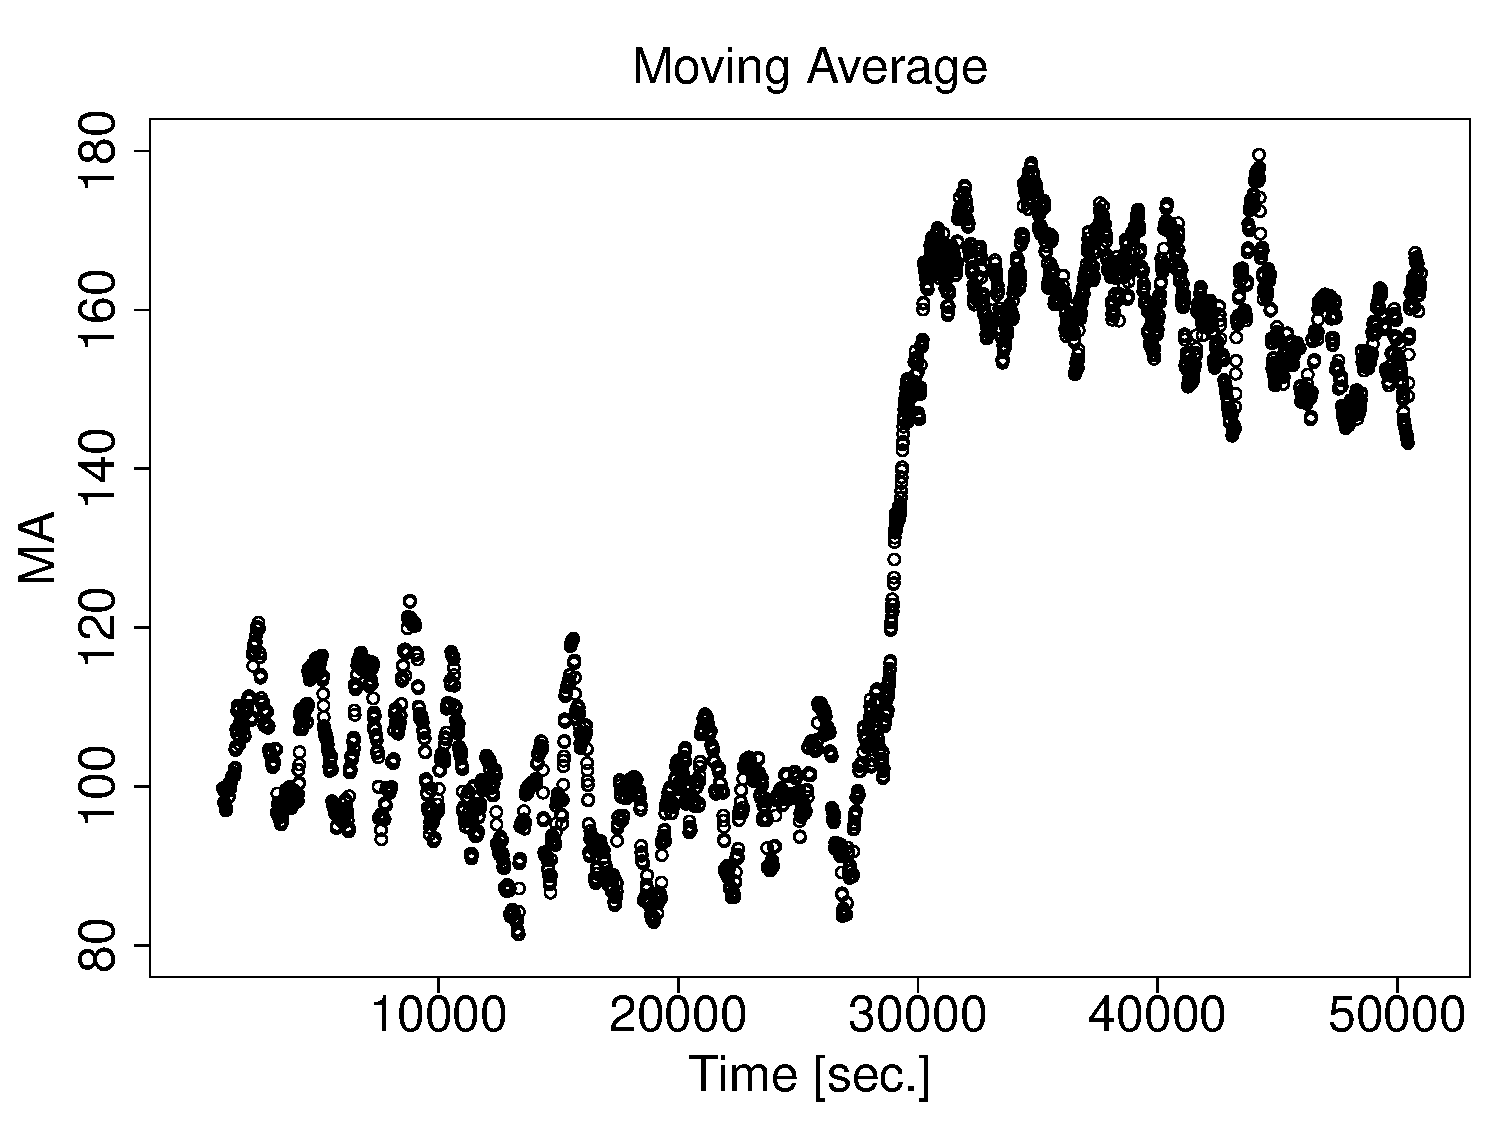
\includegraphics[width=0.45\textwidth]{pics/cfb_paper/OMF/OMFrma}
\caption{Moving average for the difference of the original signal and the fuel mass estimation.}\label{figure19}
\end{figure}
\begin{figure}[htb!]
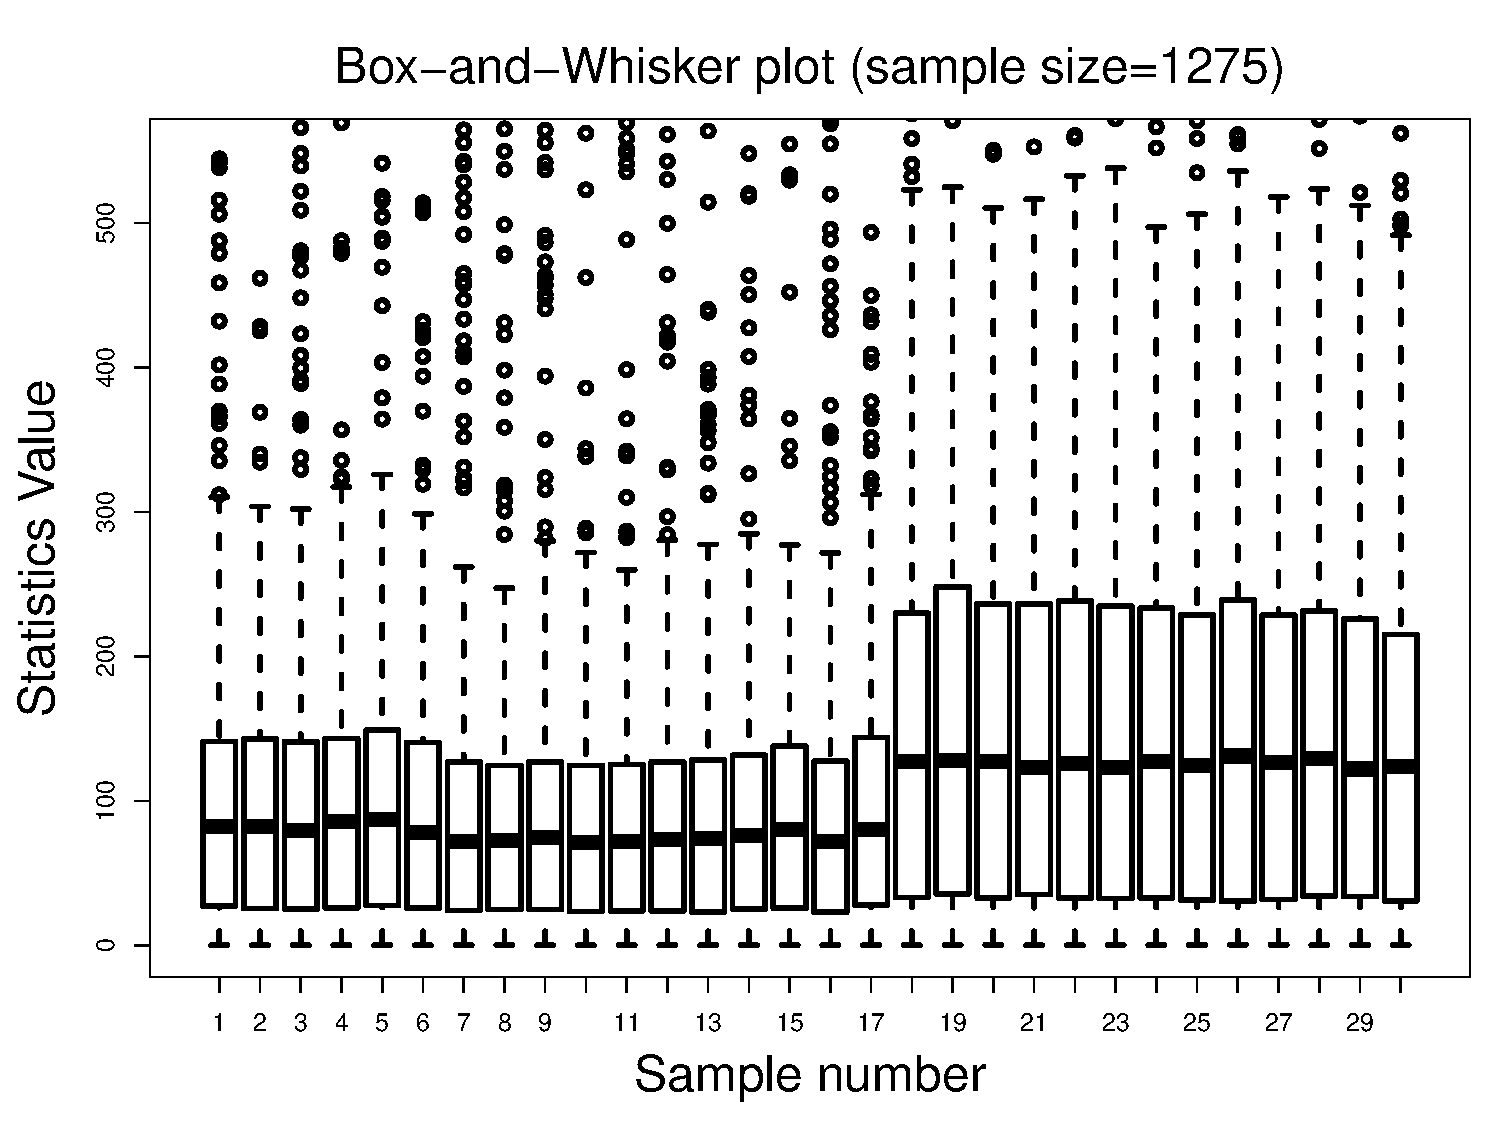
\includegraphics[width=0.45\textwidth]{pics/cfb_paper/OMF/OMFboxplot}
\caption{Box plot representing mean, lower and upper quartiles, maximum and minimum values for each of the sliding window.}\label{figure20}
\end{figure}

We could set some arbitrary limits bigger than $3\sigma$, but this may lead to overfitting if we try choosing the most appropriate limits repeating the trial and error cycles.
One way to address this problem is to handle outliers and to perform a set of a statistical test for each of the points~\cite{BakkerSensorsKDD09}.
Another way is to find a feature which is sensitive only to changes of a particular kind.
For example we can use as a feature a cumulative mean, i.e.\ average values of the signal from the beginning to the current point (Figure~\ref{figure21}).

\begin{figure}[htb!]
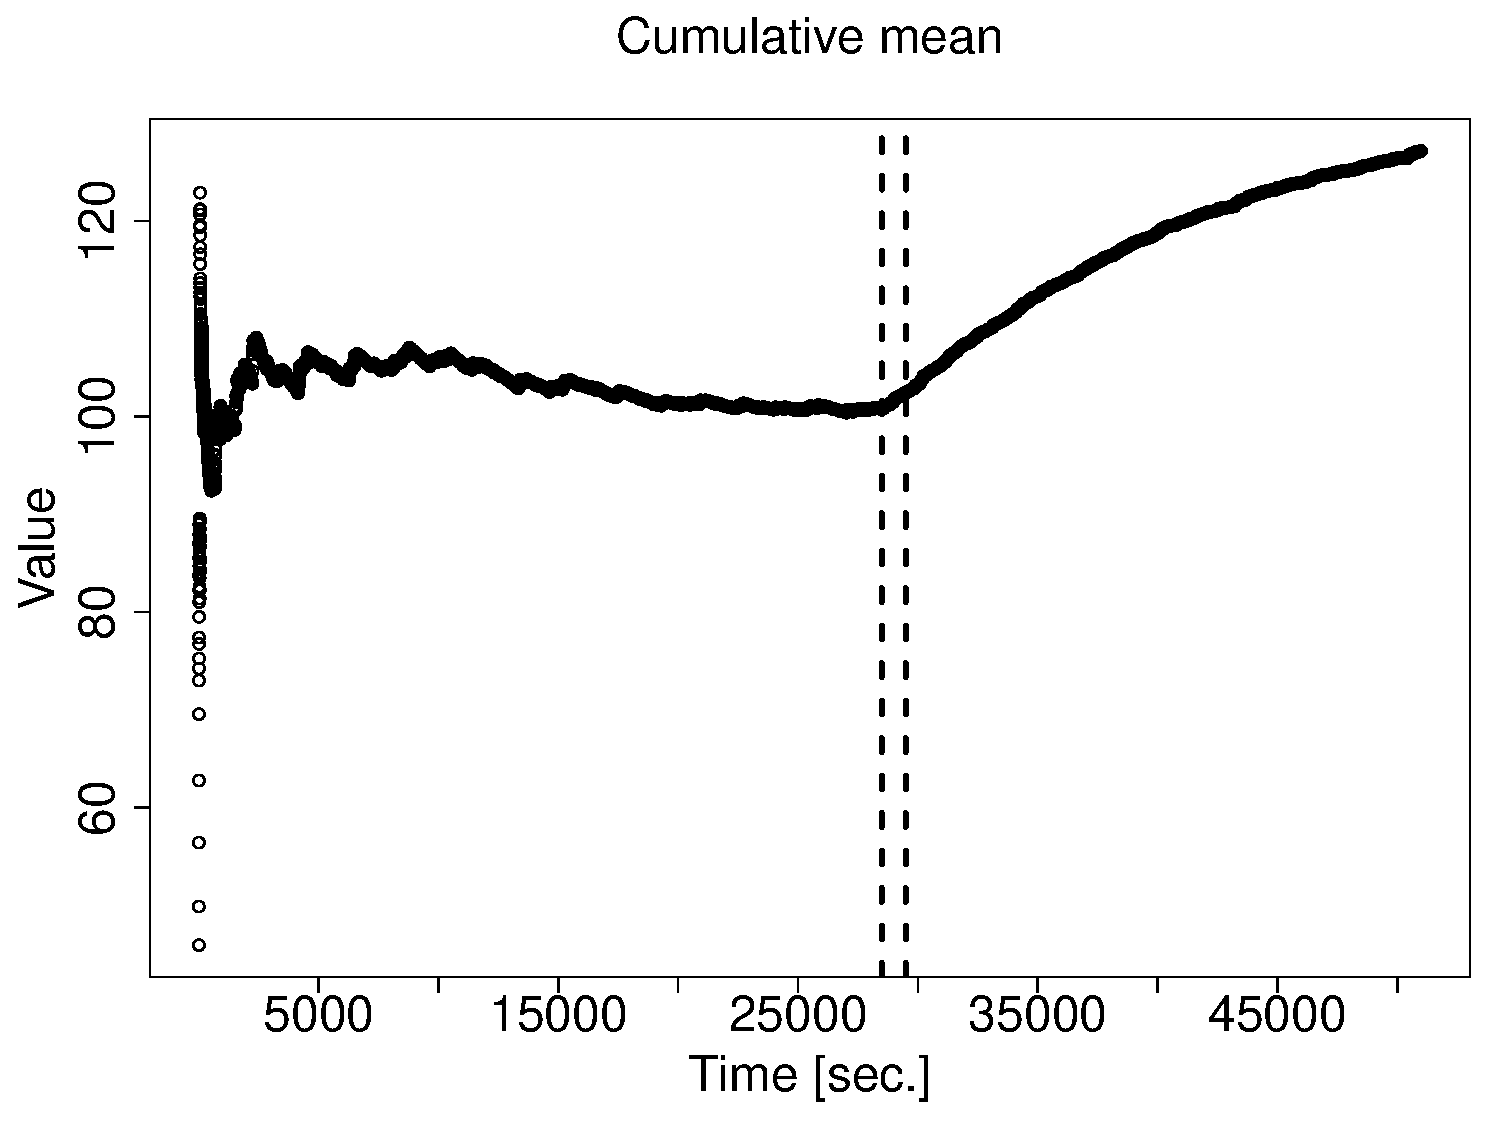
\includegraphics[width=0.45\textwidth]{pics/cfb_paper/OMF/OMFcumulativemean}
\caption{Cumulative mean}\label{figure21}
\end{figure}

In this case we can control cumulative statistic by control charts and in case of change we should calculate
this statistic from the last change point. Of course such method is computationally expensive but it is a cost to pay for the presence of the
noise and outliers.

Fortunately, QI computed on the same subset of points (from beginning of a signal to the current point) is much more resistant to outliers and noise presence.
Each time when change is detected we compute QI from the last change.
There are two parameters: the difference of logarithms of the current and the preceding values of QI and the minimum distance between changes.
With short data series, QI statistic gives statistically incorrect results.
Updates of QI were performed at the points marked by the vertical lines (Figure~\ref{figure22}).

\begin{figure}[htb!]
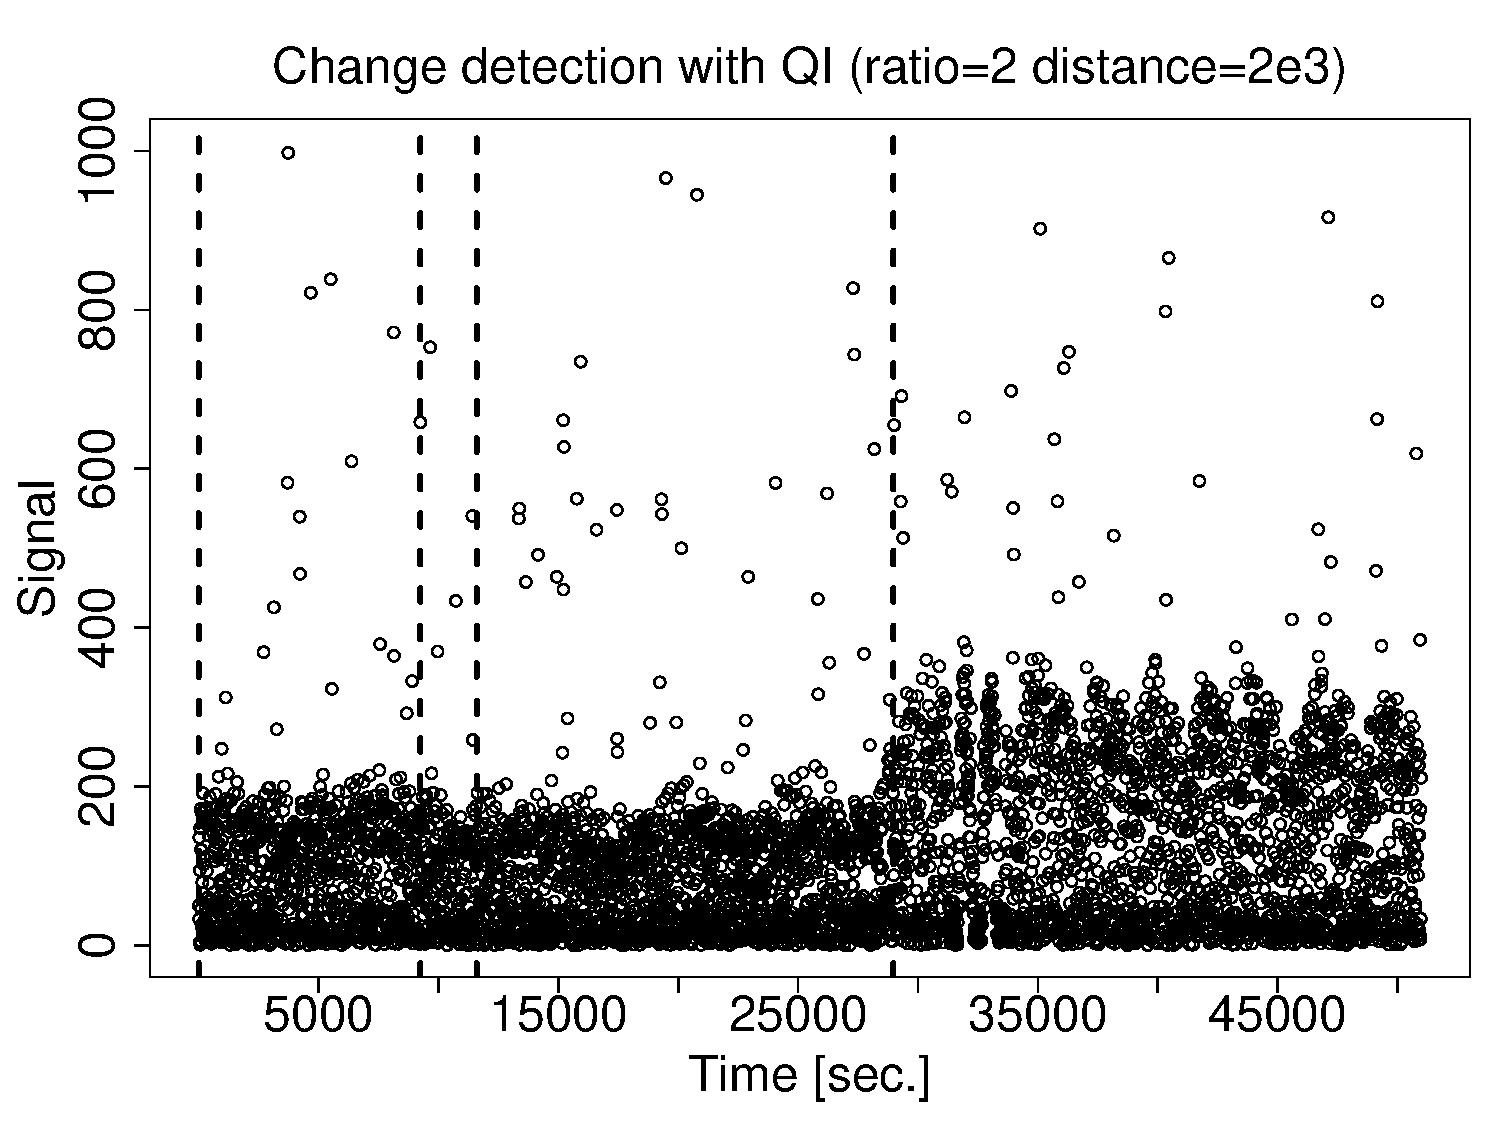
\includegraphics[width=0.45\textwidth]{pics/cfb_paper/OMF/OMFsteadyQI1}
\caption{Change points detected by means of QI which were calculated from the beginning of a signal initially and
after each detected change later. Detected points:(9236,11597,28973)}
\label{figure22}
\end{figure}

\paragraph{Detection with Density Ratio Estimation} 
Computing the density ratio estimation in the online settings (eq.~\ref{KDEformula}) we obtain change points presented in Figure~\ref{figure23}.
Actually, a series of changes is detected, but they all are concentrated near three mean points which are depicted by dashed lines.

\begin{figure}[htb!]
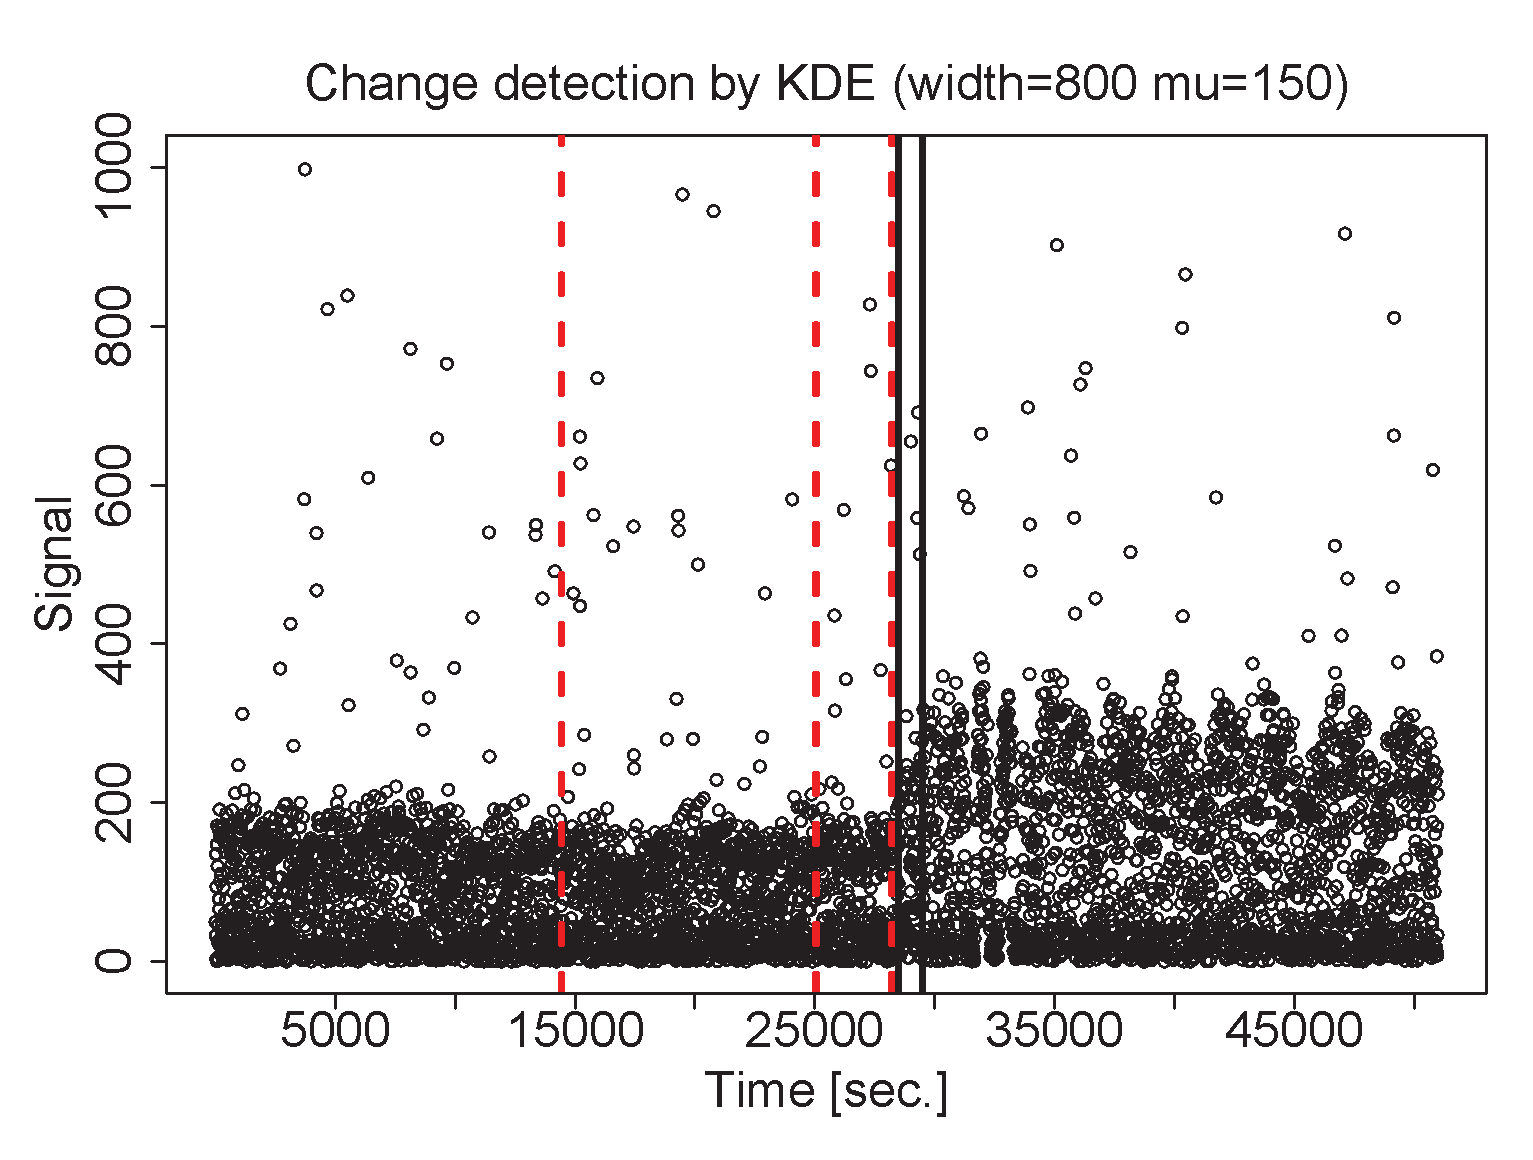
\includegraphics[width=0.45\textwidth]{pics/cfb_paper/OMF/OMFkde}
\caption{Change points detected by means KDE. Detected points:(14434,25061,28246). Successfully detected the main change at 28500 sec.} \label{figure23}
\end{figure}

\section{Conclusions}
\label{sec:conclusion}
We found a simple and intuitive approach for gradual and abrupt change detection in a noisy sensor data. 
Often sensor data needs to be preprocessed before applying change detection algorithms. For example noise and outliers should be removed.
QI-based change detection can handle gradual and abrupt changes without such preprocessing.

QI shows a good performance if the scale of a change in the mean or standard deviation
is comparable to the distance between quantiles in a test window by which we determine values of QI. 
We should note that QI shows good results for various types of changes only if sufficiently large amount of change free data from the past is available.
This is a property of the cumulative statistic.

We applied our approach for the sensor data collected from two devices modelling operation of an industrial CFB boiler. 
We analyzed different phenomena: particle size distribution and bed mass rapid change, subsequent mixture of two substances with a different PSD and mixing screw frequency change.

In the first case we had one abrupt change at the moment of adding particles with another PSD and after that the gradual
change due to mixing was following. Both kinds of changes were successfully detected by control charts, by on-line KDE and by the proposed QI method.
In the second case we attempted to detect gradual change in the fuel mass flow in a bunker, which was caused by an abrupt changes in the frequency of the mixing screw. This change was detected by means of QI and KDE.
For an abrupt change the results were similar to the case when the change happened due to the mixture of particle of different sizes.
It is interesting to note that as an aside result we found also another approach for online fuel mass estimation computing the lowest quantile.

Given these promising experimental results with QI for change detection, we plan to investigate QI further and study its behavior in a more formal and elaborate way.

\section{Acknowledgements}
This research is partly supported by Finnish Funding Agency for Technology and Innovations (TEKES) On-line CFD project and the Netherlands Organization for Scientific Research (NWO) HaCDAIS project.
Simulated sensor data were provided by VTT Research Centre of Finland.
We would like to thank R Development Core Team~\cite{Rref} and Luca Scrucca~\cite{qcc} for the open source software used in this study, \r{A}bo Akademi and Alf Hermansson for valuable technical support.

